% \setchapterimage[7.5cm]{seaside}
\setchapterstyle{kao}
\setchapterpreamble[u]{\margintoc}
%\chapter[Figures and Tables]{Figures and Tables\footnotemark[0]}
\chapter{Analyzing the relation between compositional properties and neural structures}
\labch{arithmetics}

% \cleanchapterquote{Cette langue serait merveilleuse \textup{[\,\dots]} car alors raisonner et calculer sera la même chose.}{Gottfried Wilhelm Leibniz}{Opuscules et fragments, 1890}
\cleanchapterquote{\textup{[\,\dots]}
%But the problem, you see, when you ask why something happens, 
how does a person answer why something happens? For example, Aunt Minnie is in the hospital. Why? Because she went out, slipped on the ice, and broke her hip. That satisfies people. It satisfies, but it wouldn’t satisfy someone who came from another planet and knew nothing about why when you break your hip do you go to the hospital. \textup{[\,\dots]}
% How do you get to the hospital when the hip is broken? Well, because her husband, seeing that her hip was broken, called the hospital up and sent somebody to get her. All that is understood by people. And 
when you explain a why, you have to be in some framework that you allow something to be true. Otherwise, you’re perpetually asking why. 
\textup{[\,\dots]}
%Why did the husband call up the hospital? Because the husband is interested in his wife’s welfare. Not always, some husbands aren’t interested in their wives’ welfare when they’re drunk, and they’re angry.
}{Richard Feynman}{TV program \textit{Fun to Imagine}, 1983}
% https://www.sciencealert.com/watch-richard-feynman-on-why-he-can-t-tell-you-how-magnets-work

Compositionality is thought to be a key feature of human language. Symbolic generative theories of language indeed imply the possibility of producing an infinite number of grammatical phrases and sentences using only finite means \parencite{chomsky_57, montague_70, hauser_02}. Humans derive phrase meaning by composing syntactic and semantic components using compositional rules \parencite{partee_84, cann_93, dowty_07}. % frege_1892

On the other hand, language models are trained using self-supervised objectives with no direct linguistically oriented supervision. Nonetheless, recent large pre-trained transformer models have shown striking abilities to process human language and over-perform humans on many benchmarks \parencite{devlin_19, brown_20}. They also exhibit strong consistency on agreements (subject-verb, noun-adverb, verb-verb) which are determined by abstract structures and not just linear order of words \parencite{linzen_16, gulordava_18, marvin_18, newman_21}. Yet, many studies point out that their compositional abilities are surprisingly limited and that they struggle to generalize to specific out-of-domain examples \parencite{lake_18, kim_20, hupkes_20}. 

The ability of language models to process language without inducing exhaustive symbolic composition rules is not yet fully understood. \textcite{baroni_19} suggest neural networks may process language using partially or different rules than humans. They emphasize human language is not fully characterized by algebraic rules. Language models might rely on less systematic phenomena such as semi-lexicalized constraints in syntax or irregular inflections. \textcite{lake_17} explore the possibility that language models overcome their lack of compositional abilities with an exposition to huge amounts of data.

In the previous chapters, we integrated syntactic biases into neural networks. We evaluated the use of syntactic information on meta benchmarks such as SentEval \parencite{conneau_18} or GLUE \parencite{wang_19}. However, as observed in \textcite{baroni_18}, such tasks imply various linguistic phenomenons. Although scores assess the model's ability to tackle the task, it is still unclear whether models rely on a shallow lexical pattern matching or an effective encoding of the syntactic structure and lexical information. Second, the use of large datasets for training \parencite{bowman_15, williams_18} adds difficulty in disentangling the contribution of the data from the model structure.

In this chapter, we aim at better characterizing how the model structure may affect their degree of compositionality. We first review the current methods and resources to evaluate compositionality (\refsec{composition:evaluate}). Such methods may present some limitations. In particular, they may use text-to-text setup, which makes it difficult to disentangle the effect of the encoding and decoding parts. Other methods are also sometimes focused on a limited range of linguistic phenomena. We propose two contributions in which we compare distinct structured models, including tree-shaped models and \bert. In \refsec{composition:nli}, we analyze how model structure impacts the degree of syntactic information captured by models. Using a natural language inference task, we compare the performance on sets of examples with specific linguistic properties. In \refsec{composition:arithmetic}, we intend to accurately quantify to which extent model structure is preeminent to draw compositional knowledge. We build an evaluation setup with arithmetic expressions containing specific properties. We observe how models generalize outside their domain.

% Part 2
% While transformers show outstanding performances on many NLP benchmarks, they also have some linguistic limitations. In particular, regarding their ability to generalize outside their training range and to learn elementary composition rules. The benchmark COGS \parencite{kim_20} for example highlights deep learning models struggle to generalize to longer sequences or sentences with deeper level of recursion than seen during training. 

\section{Evaluating compositionality}
\labsec{composition:evaluate}

It is undoubtedly possible to train efficient language models without prior or posterior compositional properties. Yet, building more compositional models is an active subject of research. Such methods seek to improve transformer models at learning compositional rules.
% %aims at learning true compositional rules from the training data and not just shallow surface matching pattern. 
% The gain might be to increase the model robustness toward out-of-domain examples, that is examples with statistically different properties but generated with the same set of rules.

The first step toward building such models is to provide accurate methods to measure their compositional abilities, which is notoriously hard. First—as for every other language evaluation benchmark—creating the data is a critical step. Labeling raw data is time-consuming, and it isn't easy to precisely control the examples' property. On the other hand, generating artificial data may lead to poor lexical or structural diversity. Additionally, studies show that models might use lexical biases or shallow heuristics in the data to achieve the task \parencite{linzen_18}. 

Many popular benchmarks use a text-to-text setup: models take raw text as input and should map it to a semantic form: SCAN \parencite{lake_18}, PCFG \parencite{hupkes_20}, CFQ \parencite{keysers_20} and COGS \parencite{kim_20}. For the SCAN dataset, raw sentences should be mapped to a sequence of instructions, CFQ maps sentences to Sparql queries and COGS to semantic forms.

Another line of research proposes to examine models on a natural language inference task in which the properties of sentence pairs are specified and controlled. 
\textcite{bowman_15} analyze model compositional abilities by inferring logical relations between pairs of sentences. Such sentences are artificially generated using an artificial language based on logical statements. They compare the impact of structured models to encode these sentences with explicit latent recursive structures. In our work, we try here to better characterize the effect of encoder architectures, given the various compositional aspects.
\textcite{dasgupta_18} propose a natural language inference task to evaluate the compositionality of sentences captured in embeddings. The studied properties include surface, semantic and syntactic information. % However, the range of syntactic structures and models is more limited than our proposed setup.
% \textcite{dasgupta_18} measure compositionality for sentence embeddings using a natural language inference task. They construct pairs of examples that may be solved using compositional operations. 
\textcite{mccoy_19} propose a specifically designed dataset (\textbf{HANS}) to trick models on a NLI task. Examples are designed to exhibit biases learned by statistical models. 
% Nonetheless, the paper perspective is more focus on solving such biases by modifying the training set distribution rather than model architectures. Moreover, the studied models and linguistic phenomena are rather distinct than ours.
\textcite{nie_19} aim at distinguishing the use of structure versus lexical information. Models are trained given an adversarial training setup in which object, subject, or adjectives attachment are swapped in the sentence.

Other setups exist: \textbf{PAWS} is a large dataset containing sentences that have high lexical over-lap without being paraphrases \parencite{zhang_19}. The dataset is specifically designed to distinguish models which rely on lexical heuristic to solve sematic tasks. However, they do not present a breakdown given the linguistic properties of the sentence pairs and work on binary paraphrase classification. \textcite{andreas_19} propose a formalism to measure compositionality using similarity metrics through a communication game.

Beyond evaluating the compositional capability of models, many works aim to improve them. Some methods propose to integrate structural biases within the architecture: in particular Tree-LSTM \parencite{tai_15} or in transformers with structured attention \parencite{russin_19}. Some methods also propose to adapt the pre-training or fine-tuning procedure \parencite{furrer_20}. Finally, other methods propose to complete models with modules dedicated to compositional operations \parencite{liu_20, onta_21}.

% Tree shaped models introduced in \textcite{tai_15} suggest the sentence structure could be captured directly within the model architecture. A hierarchical structure mirrored with the dependency tree could, therefore, better emphasize semantically important elements such as verbs. The system is evaluated on his ability to identify paraphrases and perform sentiment analysis. We propose to detail the model performances given the syntactic phenomenon in place.

% Regarding \bert models, \textcite{jawahar_19} analyze the properties captured in various \bert hidden layers.  Experiments do not focus on the same aspects as ours as it specifically details the difference between \bert layers with respect to more explicit linguistic phenomena detailed in probing tasks \parencite{baroni_18}. 

\section{Natural language inference}
\labsec{composition:nli}

% \bcomment{mettre un parg introductif qui dit que pour prédire l'entailment tu vas construire une représentation de chaque phrase et utiliser un module qui étant données ces représentation va prédire l'entailment en mettant les deux représentations en relation  }{}

% Toward analyzing the weaknesses of structured models for natural language inference


This chapter describes two experiments exploring whether models rely on explicit structure and compositional operations to capture sentence meaning. This section starts with analyzing the degree of syntactic information captured by structured models. We focus on a Natural Language Inference task (NLI), which aims to determine whether a given sentence entails a second. We embed both sentences from a pair using various structured models and link the embeddings using a similarity module that classifies the sentence pairs. We analyze how the sentences' specific syntactic and lexical properties impact the final performances.

We hypothesize that the complexity of the task requires a compositional aptitude to derive the general sentence meaning. However, recent work reveals that models can be easily tricked by specifically designed adversarial examples. Such examples present lexical or syntactic variations that are easily understandable for humans but result in deep confusion for statistical-based models. 
% We propose to focus on the natural language inference task, which from our hypothesis, requires an ability to perform compositional knowledge on sentences. 
To analyze the degree of syntactic information captured by structured models, we propose to evaluate a set of models on NLI examples presenting specific syntactic or lexical properties. Such an analysis grid allows us to distinguish the performance given models and linguistic phenomena. We use it to analyze how various structured models perform specific compositional operations.

%We propose an in-depth analysis to quantify the syntactic properties effectively captured by the models.  
Examples are selected given the SICK dataset \parencite{marelli_14} which consists of an NLI task specifically designed to assess model compositional properties. Samples are built to present a rich collection of linguistic constructions. Moreover, syntactic and lexical operations are designed to require specific compositional awareness. Each sentence pair is labeled given the studied transformation. We propose categorizing transformations given the induced changes on the surface lexical form or the underlying sentence structure. 

% We propose a set of designed examples to evaluate the robustness of structured models to various syntactic and lexical variations. 
% which recursively computes node representations given their children 

% \bcomment{attention orthographe et formulation}{}
Our experiments reveal that some models are indeed better adapted to capture some linguistic aspects. Moreover, we witness that some specific sentence structures or lexicon might result in severe confusion when performing inference. In particular, the replacement of words with semantic opposites or the scrambling of words between the premise and hypothesis. For the latter, we perform additional analysis to better capture the inclination of models to generalize in such complex linguistic structures. We show that, while some cases might be addressed by carefully choosing the model structure, for others, it seems the relation of entailment can only be learned by augmenting the training set with corresponding examples.

%%%%%%%%%%%%%%%%%%%%%%%%%%%%%%%%%%%%%%%%%%%%%%%%%%%%%%%%%%%%%%%%%%%%%%%%%%%%%
\subsection{Method}
\labsec{composition:nli:mehtod}

% \begin{figure*}[!htb]
% \begin{center}
% \includegraphics[width=15cm]{figures/model-all.png}
% \end{center}
% \caption{\textbf{Sentences encoder architecture:} We use Bert in a \textit{fine-tuning} configuration such that the final output layer is used as input for a structured model as proposed in the Section \ref{sec:studied-structures}.}
% \label{fig:model-all}
% \end{figure*}
% \FloatBarrier

We map sentences $s$ to embeddings $h_s$ using the models exposed in \refsec{survey:encoding}: Bag Of Word (\bow), sequential LSTM (\seq),  hierarchical models such as Tree LSTM for dependency and constituency structure (\dep and \const) and \bert (\cls).

% \bcomment{why dependency trees here ? it is not clear how do these trees are used, the picture is insufficient}{}
Regarding the Tree LSTM  models, we obtain the dependency structures using the deep biaffine parser from \textcite{dozat_17} and the constituency structures using the constituency neural parser from \textcite{klein_18}. Regarding \bert, we use the original \bert-base and the \cls token as the sentence embedding. 

For each model, we consider two types of embeddings vectors. We use either traditional GloVe embeddings \parencite{pennington_14} or, as illustrated in \reffig{model}, contextualized vector from \bert model \parencite{devlin_19}. When using \bert as embedding, vectors are normalized with the L2 norm for \bow model to facilitate the joint convergence of the model and \bert layers. When using GloVe embeddings, we used 300-dimensional word vectors trained on the common crawl dataset (840B tokens) with a vocabulary of 2.2M case-sensitive words.
% All models are detailed bellow:

\begin{figure}[!htb]
\begin{center}
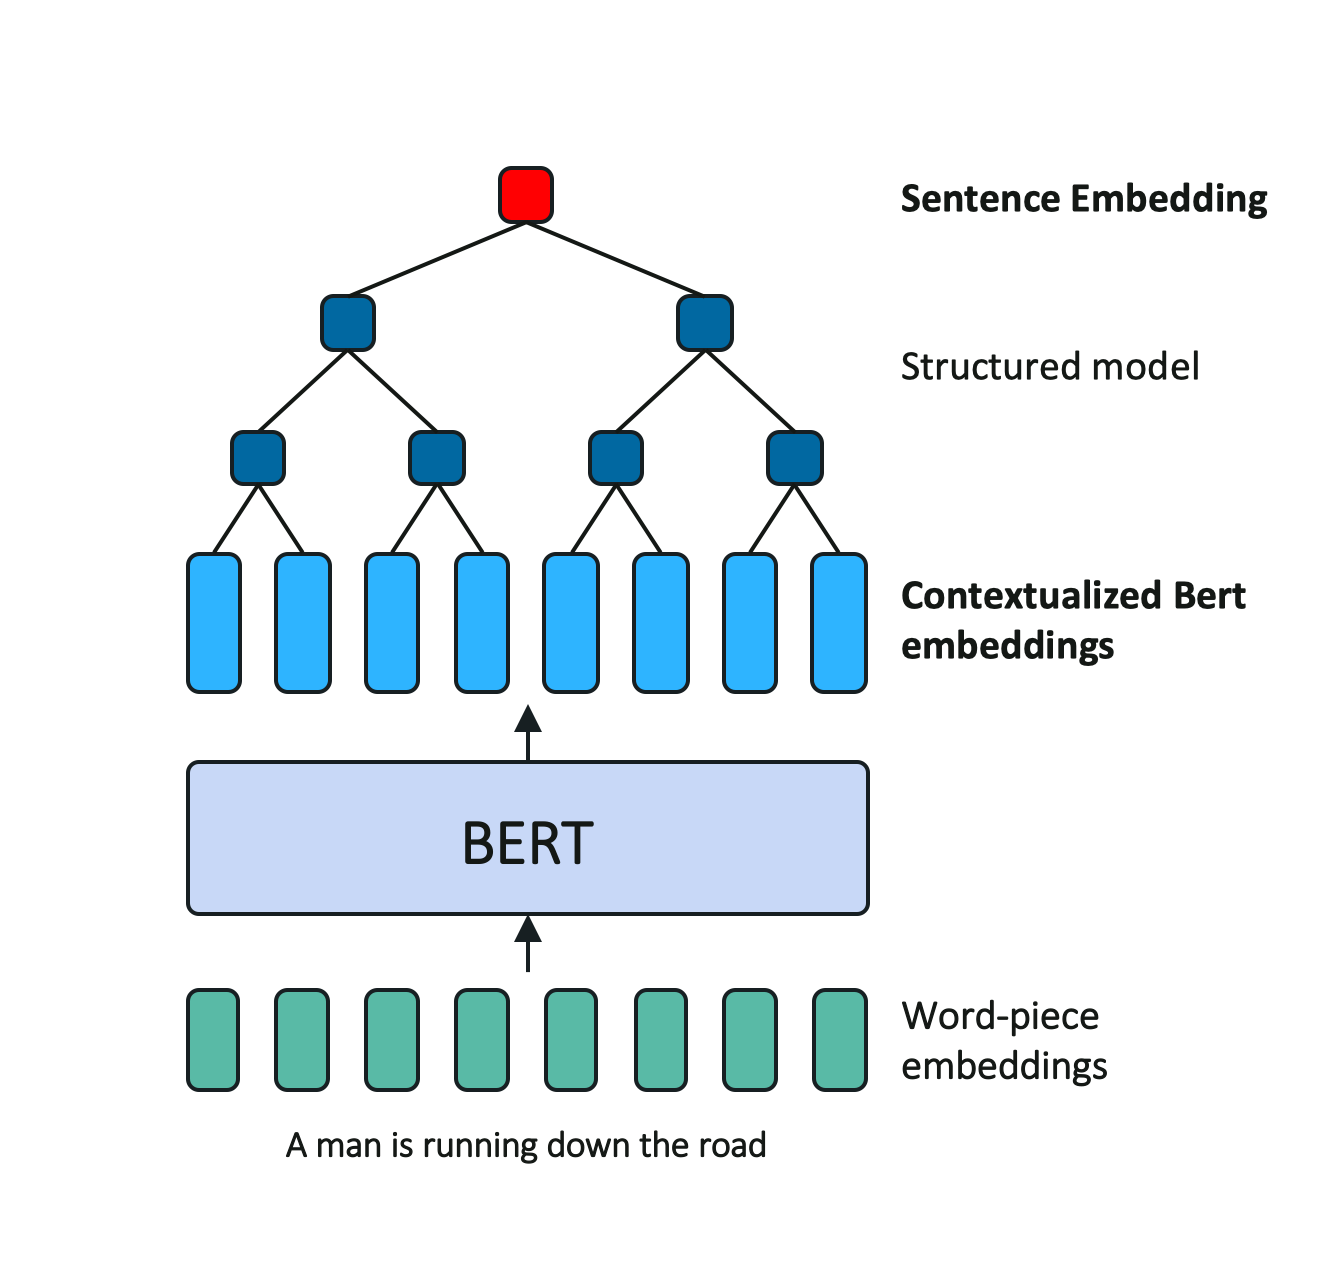
\includegraphics[width=7cm]{images/model-struct.png}
\end{center}
\caption{Models architecture: We use either GloVe static embedding or \bert in a \textit{fine-tuning} configuration such that the final output layer is used as input for a structured model as detailed in the \refsec{composition:nli:mehtod}.}
\labfig{model}
\end{figure}

\subsubsection{Similarity architecture and training objective}
\label{sec:training-setup}
%4500/500/4927 
We choose a similar supervised framework as in \textcite{tai_15} and use the given train/dev/test split. We illustrate the full model in \reffig{similarity}. Parameters are set given results on the dev set, and results are presented on the test set. In the experiments section, results are presented given the transformation applied to each couple of sentences. 

% For the SICK-E task, the target distribution is defined as 3-dimensional one-hot vector:

% \begin{equation*}
% p = \left\{
% \begin{array}{ll}
% $[1, 0, 0]$, & \text{Entailment} \\
% $[0, 1, 0]$, & \text{Contradiction} \\
% $[0, 0, 1]$, & \text{Neutral}
% \end{array} \right.
% \end{equation*}

% We transform the target $y$ from the SICK-R task into the distribution $p$ defined by:

% \begin{equation*}
% p_{i} = \left\{
% \begin{array}{ll}
% y - \lfloor{y}\rfloor, & i = \lfloor{y}\rfloor + 1 \\
% \lfloor{y}\rfloor - y + 1, & i = \lfloor{y}\rfloor \\
% 0 & \text{otherwise}
% \end{array} \right.
% \end{equation*}

Regarding \bert, we do not use the similarity architecture, bu rather directly fed the sentence pair to \bert. The prediction is based on the \cls token, later processed by a linear layer and a softmax activation function.

For other encoders, a dedicated architecture predicts the similarity distribution of a pair of sentences. The similarity module takes as input a pair of sentence vectors ($h_{L}, h_{L})$ and computes their component\-wise product $h_{L} \odot h_{R}$ and their absolute difference $|h_{L} - h_{R}|$. These features are then fed to a two layers perceptron network (MLP) to compute the probability distribution  $\hat{p}_{\theta}$:
\begin{align}
\begin{split}
&h_{\times}=h_L\odot h_R, ~~~~~h_{+} = |h_L - h_R |, \\
&h_s = \sigma (W^{(\times)}h_{\times} + W^{(+)}h_{+} + b^{(h)}), \\
&\hat{p}_{\theta} = \softmax(W^{(p)}h_s + b^{(p)}),\\
\end{split}
\end{align}

The KL-divergence between the predicted distribution $\hat{p}_{\theta}$ and the ground truth $p$ is used as training objective:
\begin{equation}
J(\theta) = \frac{1}{N}\sum_{k=1}^{N}\text{KL}(p^{(k)} \Big|\Big| \hat{p}_{\theta}^{(k)}) + \frac{\lambda}{2}||\theta||_{2}^{2}
\end{equation}

The ground truth $p$ is a three-dimensional one-hot vector defined given the relation between the two sentences in the pair (entailment, contradiction, or neutral). During inference, the argmax of $\hat{p}$ is considered. We report the accuracy between targets and predictions to evaluate the performances.
% for the SICK-R task, the similarity score $\hat{y}$ is computed by $\hat{y} = r^{\intercal} \hat{p}_{\theta}$ with $r^{\intercal} = [1, \dots, 5]$.

% For each image in the original data set, three captions are written by human. For each given sentence, a set of syntactically modified sentences is generated. For each image, two random sentences are paired. They can be issued from two different human-generated captions or from the same original caption but with artificial modifications. For each pair, only one sentence may be transformed. We classify pairs given the transformations performed on one sentence from each pair. In particular, we analyze the robustness of the model to such transformations.

% We classify the transformations into three categories. Each category of alteration induces changes on the surface form of the sentence but local changes with respect to a given underlying structure. Categories are defined given the considered modifications and associated structure.

\begin{figure}[!htb]
\begin{center}
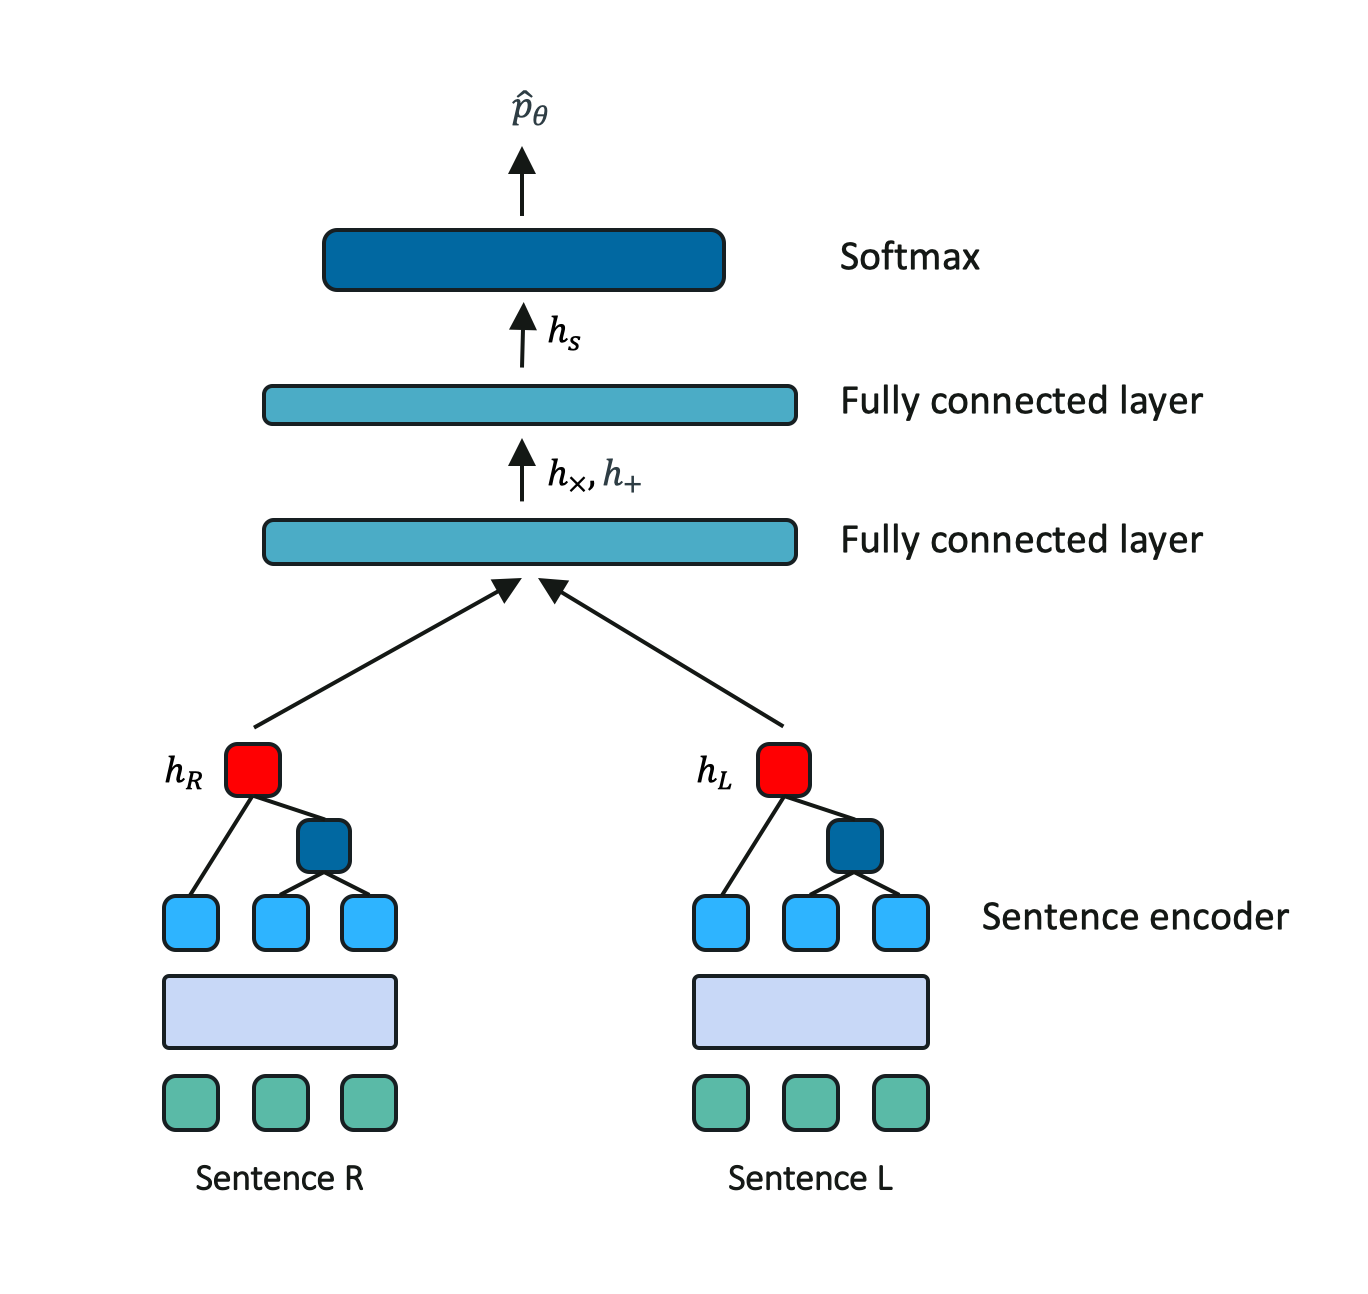
\includegraphics[width=9cm]{images/similarity.png}
\end{center}
\caption{We embed sentences using various structured models. The similarity architecture uses the sentence embeddings component-wise product and absolute difference to output a probability distribution for the entailment label.}
\labfig{similarity}
\end{figure}

\subsubsection{Hyper parameters setting}

% and differentiate the training parameters between bert layers and other layers
Parameters are fixed using the dev set. We use a 25 batch size. We use the \bert-base-cased model \parencite{wolf_19} with an embedding size of 768. For \bert layers, we use 0.10 weight decay and fix the learning rate to 2e-5. For other layers, the learning rate is fixed to 0.025 with a weight decay of 1e-4. Layers are initialized using a glorot distribution \parencite{glorot_10} . Biases are initially set to 0 for tree structure models and 1 for \seq model. When applicable, the model hidden-size is fixed to respectively 150 and 300 when using GloVe and \bert emeddings. The hidden-size of the similarity module is set to 50. Models are trained during a maximum of 20 epochs using the Adagrad optimizer \parencite{duchi_11} and AdamW for \bert \parencite{loshchilov_19}. When no improvement is observed on the dev set for 3 consecutive epochs, the training is stopped. Results are reported on the test set. 
% The gradient is clipped to the standard value of 5.
% We also impose a warm-up profile: The learning rate is set to zero during the first epoch, linearly increase during the epoch 2 and 3 and then is kept to 5e-5. For other layer, the warm-up profile impose a linear increase during the first epoch.
% Xavier init procedure?
% Adgrad optimizer 
% 
%%%%%%%%%%%%%%%%%%%%%%%%%%%%%%%%%%%%%%%%%%%%%%%%%%%%%%%%%%%%%%%%%%%%%%%%
\subsection{Linguistic phenomena experiment}
\label{sec:linguistic-breakdown}

% In this section we train our model on the SICK \parencite{marelli_14} and HANS dataset \parencite{mccoy_2019}. Both are NLI dataset where for each sentence pair a specific linguistic property is studied. The SICK dataset contains 9840 sentence pairs and the HANS dataset, 30000. The SICK dataset already propose a train/dev/test split. For the HANS dataset, we manually applied a stratified shuffle split given the linguistic transformations. Each set represent respectively 40/50/10 percent of the original dataset.

\subsubsection{SICK Data} 

\begin{table*}[!htb]
\footnotesize
\centering
\begin{tabularx}{16cm}{@{}c l Y Y@{}}
\toprule
\multicolumn{2}{c}{\textbf{Transformations}} &  \multicolumn{2}{c}{\textbf{Examples}}\\\midrule
\multicolumn{4}{c}{\textit{Lexical transformations}}\\\midrule
\textbf{null} & No transformation & Three boys are jumping in the leaves & Children in red shirts are playing in the leaves \\
\textbf{so} & Replace words with semantic opposites & A \textbf{man} is rowing a boat & A \textbf{woman} is rowing a boat\\
\textbf{lex} & Replace words with synonyms & A young \textbf{boy} is jumping into water & A young \textbf{kid} is jumping into water\\
\textbf{det} &  Replace quantifiers & \textbf{The} surfer is riding a big wave & \textbf{A} surfer is riding a big wave\\\midrule
\multicolumn{4}{c}{\textit{Syntactic clauses expansion}}\\\midrule
\textbf{aa} & Add modifiers &  A deer is jumping a fence & A \textbf{wild} deer is jumping a fence\\
\textbf{expn} & Expand agentive nouns & \textbf{Some people playing rugby} are tackling each other & \textbf{Rugby players} are tackling each other\\
\textbf{expa} & Turn adjectives into relative clauses & A \textbf{cute} panda is lying down & A panda \textbf{that is cute} is lying down\\
\textbf{expc} &  Turn compounds into relative clauses & The woman is frying a \textbf{chop of breaded pork} & The woman is frying a \textbf{breaded pork chop}\\\midrule
\multicolumn{4}{c}{\textit{Global transformations}}\\\midrule
\textbf{od} & Change determiners with opposites &  \textbf{A} dog is barking & \textbf{There is no} dog barking\\
\textbf{inv} & Insert a negation & The boy is playing the piano & The boy is \textbf{not} playing the piano\\
\textbf{top} & Turn active sentences into passive & A man is driving a car & The car is being driven by a man\\
\textbf{ws} & Scramble words & The \textbf{turtle} is following the \textbf{fish} & The \textbf{fish} is following the \textbf{turtle}\\
\bottomrule
\end{tabularx}
\caption{Sick expansion rules: Detailed transformations applied to generate the SICK dataset. Transformations are categorized given their impact on the sentence surface form. The null transformation refers to sentence pairs for which no expansion transformation was performed: we only pair two normalized sentences describing the same picture in the original dataset. For every other transformations, the final sentence pair is generated out of a single original sentence transformed with normalization and expansion operations.}
 \label{table:sick}
\end{table*}

% \sidenote{The dataset distribution is unbalanced regarding the applied transformations. In particular, some transformations only concern a small proportion of samples. This is specifically the case of the \textbf{expn} expansion with only 13 samples in the test set. We observed a high standard variation between runs for this category. To present a statistically more valid interpretation, we add some additional examples for \textbf{expn}. We introduce a heuristic to generate example sentences in which we expand nouns into more complex expressions. In particular, we use wordnet \parencite{miller_95} to replace nouns with expended nominal groups. For example, we replace the word "doctors" with the expression "licensed medical practitioners". We add a total of 152 examples distributed in each split for the \textbf{expn} transformation.}
The SICK dataset \parencite{marelli_14} consists of \numprint{9840} sentence pairs which have been manually annotated to assess whether the first entails the second. The original sentences are sampled from the 8K Image Flickr dataset \cite{dhodosh_13} and the SemEval 2012 STS MSR Video Description dataset \cite{agirre_12}. These two datasets contain sentences describing the same picture or video. The sentence pairs are then transformed through a 3-steps process: normalization to remove unwanted linguistic phenomena; expansion to obtain sentences with specific characteristics; pairing expanded sentences with normalized sentences (and pairing both normalized sentences from the pair).
The dataset is already split into train/dev/test containing respectively \numprint{4506}/\numprint{505}/\numprint{4979} samples. Sentence pairs have been manually transformed to include specific syntactic or lexical properties detailed in Table \ref{table:sick}. The dataset is freely available for research purposes\sidenote{\url{https://zenodo.org/record/2787612\#.Xjh2qxfjJ24}}. Moreover, some additional indexes detail the transformation that was applied to one of the sentences from each pair. We use this information to perform a detailed breakdown of the performance of various models given the transformation. We divide the transformations into three categories, given the degree of induced alteration on the sentence surface form.

\begin{itemize}
    \item \textbf{Lexical transformations} The first set of transformations induces local changes. Only individual words are modified. Given the modification, the sentence meaning can be preserved or altered. We expect every model to be robust to such changes. 
    \item \textbf{Syntactic clauses expansion} In this set of alterations, we add, remove or modify sub-trees of the sentence structure. Such transformation has a low impact on the syntactic tree structure but can deeply transform the surface form of the sentence. We expect strongly structured models to be more robust to such transformations.
    \item \textbf{Global transformations} Finally, we consider a set of modifications that impact both the surface and syntactic form.
\end{itemize}

We also considered the possibility of exploiting the HANS dataset \parencite{mccoy_19}, which gathers \numprint{30000} sentence pairs automatically generated with specific linguistic properties. Similarly to the SICK dataset, HANS aims at identifying models relying on shallow heuristics to perform natural language inference and includes a larger set of transformations. However, it does not aim to characterize model compositional abilities, as it generates sentences based on a set of templates that share a similar compositional scheme. From our point of view, it is less adapted for a fine grained analysis of compositional knowledge.
% The proposed categories are developed below. 
% The sentences are sampled from two datasets, the 8K ImageFlickr data set \parencite{dhodosh_15} and the SemEval 2012 STS MSR- Video Description data set \parencite{agirre_12}. standardization and syntactic or lexical specific transformations.

% \subsection{Studied transformations}

% \paragraph{Lexical transformations} The first set of transformations induces local changes. Only individual words are modified. Given the modification, the sentence meaning can be preserved or altered. We expect every model to be robust to such changes. 
% The set of transformations is detailed below:

% \begin{itemize}
%     \item \textbf{null} No transformation.
%     \item \textbf{so} Replace words with semantic opposites. Example: "The girl is spraying the plants with water" $\rightarrow$ "The boy is spraying the plants with water"
%     \item \textbf{lex} Replace words with synonyms. Example: "A young boy is jumping into water" $\rightarrow$ "A young kid is jumping into water"
%     \item \textbf{det} Replace quantifiers. Example: "The surfer is riding a big wave" $\rightarrow$ "A surfer is riding a big wave"
% \end{itemize}

% \paragraph{Syntactic clauses expansion} In this set of alterations, we add, remove or modify sub-trees of the sentence structure. such transformation has a low impact on the syntactic tree structure but can deeply transform the surface form of the sentence. We expect strongly structured models to be more robust to such transformations.
% The set of transformations is detailed below:

% \begin{itemize}
%     \item \textbf{aa} Add modifiers. Example: "A deer is jumping a fence" $\rightarrow$ "A wild deer is jumping a fence"
%     \item \textbf{expn} Expand agentive nouns. Example: "A soccer player is kicking a ball into the goal" $\rightarrow$ "A person who plays soccer is kicking a ball into the goal"
%     \item \textbf{expa} Turn adjectives into relative clauses. Example: "Two men are taking a break from a trip on a snowy road" $\rightarrow$ "Two men are taking a break from a trip on a road covered by snow"
%     \item \textbf{expc} Turn compounds into relative clauses. Example: "A woman is using a sewing machine" $\rightarrow$ "A woman is using a machine made for sewing"
% \end{itemize}

% \paragraph{Global transformations} Finally, we consider a set of modifications that impact both the surface and syntactic form.
% The set of transformations is detailed below:

% \begin{itemize}
%     \item \textbf{od} Change determiners with opposites. Example: "A dog is walking along a snowdrift" $\rightarrow$ "There is no dog walking along a snowdrift"
%     \item \textbf{inv} Insert a negation. Example: "The boy is playing the piano" $\rightarrow$ "The boy is not playing the piano"
%     \item \textbf{top} Turn active sentences into passive. Example: "A man is driving a car" $\rightarrow$ "The car is being driven by a man"
%     \item \textbf{ws} Scramble words. Example: "The turtle is following the fish" $\rightarrow$ "The fish is following the turtle"
% \end{itemize}

% \subsection{Linguistic properties breakdown} 
% \label{sec:model-type}


%%%%%%%%%%%%%%%%%%%%%%%%%%%%%%%%%%%%%%%%%%%%%%%%%%%%%%%%%%%%%%%%%%%%%%%%
% \FloatBarrier
\subsubsection{Lexical transformations} 

% \bcomment{un peu curieux ce style}{}

In the following sections, we compare how structured models behave when facing such sets of transformations. Results for lexical transformations are reported in Table \ref{table:results-local}. We observe a distinction between \textbf{so} and \textbf{lex} transformations which replace individual words with respectively antonyms or synonyms. For \textbf{so} transformations, models show difficulty in propagating lexical transformation into the final sentence embedding and adjusting the meaning of the sentence. For \textbf{so} transformations, we also observe that the use of contextualized embeddings seems to even lower the results of structured models compared to the use of static GloVe embeddings.
% While both transformations are rather technically similar, the impact on the power of prediction of models is different. 
% When using GloVe embeddings, all models have better performances when predicting meaning preserving transformation, except for the dependency structure.  Finally for the \textbf{det} transformation, only the baseline Bag Of Words model is impacted and all models shows a strong robustness to quantifier transformations.


\begin{table*}[!htb]
\footnotesize
% \begin{minipage}{\textwidth}
\centering
\begin{tabularx}{16cm}{@{}c Y Y Y Y @{}}
\toprule
 & \textbf{No transformation (null)} & \textbf{Replace words with semantic opposites (so)} & \textbf{Replace words with synonyms (lex)} & \textbf{Replace quantifiers (det)}\\\midrule
 N & \numprint{2558} & \numprint{461} & \numprint{399} & \numprint{118}\\\midrule\multicolumn{5}{c}{\textit{Glove embeddings}}\\\midrule
\bow & 81.6 \scriptsize{(0.9)} & 49.3 \scriptsize{(3.6)} & 57.3 \scriptsize{(2.7)} & 82.0 \scriptsize{(5.1)}\\
\const & 84.6 \scriptsize{(0.2)} & 66.5 \scriptsize{(2.5)} & 76.5 \scriptsize{(1.6)} & 98.6 \scriptsize{(0.9)}\\
\seq & 83.1 \scriptsize{(1.2)} & 63.7 \scriptsize{(6.8)} & 74.1 \scriptsize{(3.9)} & \textbf{98.8} \scriptsize{(0.9)}\\
% \seq (uni) & 81.2 \scriptsize{(0.7)} & 62.0 \scriptsize{(1.2)} & 69.4 \scriptsize{(5.2)} & 82.9 \scriptsize{(10.5)}\\
\dep & \textbf{84.8} \scriptsize{(0.5)} & \underline{\textbf{69.6}} \scriptsize{(1.2)} & \textbf{76.5} \scriptsize{(2.4)} & 98.6 \scriptsize{(0.7)}\\
\midrule\multicolumn{5}{c}{\textit{\bert embeddings}}\\\midrule
\bow & 77.5 \scriptsize{(1.2)} & 26.9 \scriptsize{(6.0)} & 80.2\scriptsize{(4.3)} & 93.6 \scriptsize{(5.9)}\\
\const & 76.0 \scriptsize{(2.7)} & 53.6 \scriptsize{(3.5)} & 77.8 \scriptsize{(3.0)} & 96.8 \scriptsize{(2.4)}\\
\seq & 81.5 \scriptsize{(1.3)} & 46.9 \scriptsize{(3.3)} & \underline{\textbf{83.6}} \scriptsize{(2.1)} & \underline{\textbf{100.0}} \scriptsize{(0.0)}\\
% \seq (uni) & 81.2 \scriptsize{(2.3)} & 44.5 \scriptsize{(5.9)} & \underline{\textbf{81.7}} \scriptsize{(2.4)} & 99.0 \scriptsize{(1.6)}\\
\dep & 82.7 \scriptsize{(0.9)} & 57.6 \scriptsize{(2.0)} & 80.8 \scriptsize{(1.2)} & 99.3 \scriptsize{(0.6)}\\
\cls & \underline{\textbf{86.1}} \scriptsize{(1.4)} & \textbf{68.8} \scriptsize{(7.4)} & 77.4 \scriptsize{(3.6)} & 98.3 \scriptsize{(0.9)}\\
% N & 2787 & 473 & 407 & 121\\\midrule\multicolumn{5}{c}{\textbf{Glove embeddings}}\\\midrule
% \bow & 80.9 \scriptsize{(0.8)} & 45.1 \scriptsize{(6.2)} & 62.9 \scriptsize{(4.9)} & 85.3 \scriptsize{(5.1)}\\
% \const & 83.8 \scriptsize{(0.8)} & 65.2 \scriptsize{(2.8)} & 73.4 \scriptsize{(4.2)} & 98.5 \scriptsize{(1.1)}\\
% \seq & 85.1 \scriptsize{(0.4)} & 67.2 \scriptsize{(2.2)} & \textbf{80.0} \scriptsize{(2.6)} & \textbf{99.3} \scriptsize{(0.6)}\\
% \dep & \textbf{85.2} \scriptsize{(0.6)} & \underline{\textbf{69.5}} \scriptsize{(1.5)} & 75.8 \scriptsize{(2.4)} & 98.7 \scriptsize{(0.8)}\\
% \midrule\multicolumn{5}{c}{\textbf{Bert embeddings}}\\\midrule
% \bow & 85.6 \scriptsize{(0.6)} & 59.1 \scriptsize{(0.8)} & \underline{\textbf{83.1}} \scriptsize{(1.2)} & 99.7 \scriptsize{(0.7)}\\
% \const & 83.8 \scriptsize{(0.3)} & 64.4 \scriptsize{(2.2)} & 80.8 \scriptsize{(1.3)} & \underline{\textbf{99.8}} \scriptsize{(0.3)}\\
% \seq & 85.5 \scriptsize{(0.6)} & 62.6 \scriptsize{(1.8)} & 81.7 \scriptsize{(1.6)} & 99.5 \scriptsize{(0.7)}\\
% \dep & 85.8 \scriptsize{(0.6)} & \textbf{68.9} \scriptsize{(1.1)} & 80.4 \scriptsize{(2.1)} & 99.7 \scriptsize{(0.4)}\\
% \cls & \underline{\textbf{87.0}} \scriptsize{(0.6)} & 58.6 \scriptsize{(3.9)} & 78.3 \scriptsize{(4.2)} & 98.3 \scriptsize{(1.7)}\\
\bottomrule
% \toprule
%  & \textbf{null} & \textbf{so} & \textbf{lex} & \textbf{det}\\\midrule
% N & 2787 & 473 & 407 & 121\\\midrule
% Dependency & 85,15 & \textbf{72,73} & 70,52 & 99,17\\
% Constituency & 84,18 & 68,5 & 72,97 & 97,52\\
% Sequence (BERT) & \textbf{87,94} & 64,48 & \textbf{79,85} & \textbf{100,00}\\
% Sequence (GRU) & 84,61 & 70,4 & 72,48 & \textbf{100,00}\\
% Bag Of Words & 82,63 & 52,01 & 55,04 & 81,82\\
% \bottomrule
\end{tabularx}
\caption{Accuracy on the test set for SICK-E task for pair samples with lexical transformations. We report a mean over 5 runs (standard deviations in parentheses). The best results for a given embedding are in \textbf{bold}. The best results overall are \underline{underlined}. The null transformation consider pair obtained out of two different original sentences. The two sentences can differ given multiple, uncontrolled lexical or syntactic phenomena. Therefore, the performances are usually lower for this category.}
 \label{table:results-local}
 %  
%  \end{minipage}
\end{table*}


% \bcomment{que représentent les colonnes null et det, j'ai du mal à interpréter les chiffres}{}
\paragraph{Models may be sensible to lexical variations}

Some pairs seem difficult to predict for \cls and \bow models. For example, the following sentence pair is almost systematically wrongly classified on all five runs: "A little \textbf{boy} and a woman wearing a yellow shirt are getting splashed by a city fountain" $\rightarrow$ "A little \textbf{girl} and a woman wearing a yellow shirt are getting splashed by a city fountain". For \bow, we can extrapolate that the fact that the subject includes two people induces some confusion in the output representation. It is less clear for \cls.

% Some interesting mistakes include the behavior of models when performing \textbf{so} transformations. 
The \dep model seems particularly sensitive to transformations operated on the sentence's main verb. For example, the following sentence pair is better classified by \dep and \seq models:
"A woman is \textbf{applying} cosmetics to her eyelid" $\rightarrow$ "A woman is \textbf{removing} cosmetics from her eyelid".

% "The little dog is \textbf{dropping} the bedroom slipper from its mouth" $\rightarrow$ "The little dog is \textbf{grabbing} the bedroom slipper with its mouth", 

% On the contrary, for the following sentence pair, only the dep model is having trouble predicting the correct label. "Two men, a woman, and two young boys are \textbf{sitting} in front of a large gathering of people outside a building" $\rightarrow$ "Two men, a woman, and two young boys are \textbf{standing} in front of a large gathering of people outside a building"

% \FloatBarrier
\subsubsection{Syntactic clauses expansion}


% \bcomment{aider le lecteur}{rappeler ce que sont aa, expn etc}
% For syntactic clauses expansion, all transformations preserve the sentence final meaning.
% Constituency structure seems well suited for the expansion of agentive nouns (\textbf{expn}). 
% For this set of transformation, we expect structured models such as Tree LSTM to be more robust to such transformations. However, when looking into details, the impact of the model's underlying structure depends on the transformation. 
This set gathers transformations involving syntactic expansion. All models show a strong robustness to adding modifiers (\textbf{aa} expansion). When only using GloVe embeddings, expanding agentive nouns (\textbf{expa}), turn adjectives into relative clauses (\textbf{expn}) and turning compounds into relative clauses (\textbf{expc}) expansions seem to be better captured by tree-structured model. However, using \bert embeddings reduces the gap between models, which suggests some syntactic information is captured in contextualized embeddings for such transformations. It is particularly explicit for the \bow model as the performance using GloVe or \bert word embedding deeply differs for all transformations. 

% \textbf{expa} transformations which turn adjectives into relatives clauses are better handle by \seq when using GloVe embeddings. However, the initialization with contextualized embeddings benefit to the \seq model which outperform the simple \cls model on both \textbf{expn} and \textbf{expa}.
% On the contrary, we expect such transformation to be challenging for a model which do not assume a complex underlying structure. 

\begin{table*}[!htb]
\footnotesize
% \begin{minipage}{\textwidth}
\centering
\begin{tabularx}{16cm}{@{}c Y Y Y Y @{}}
\toprule
 & \textbf{Add modifiers (aa)} & \textbf{Expand agentive nouns (expn)} & \textbf{Turn adjectives into relative clauses  (expa)} & \textbf{Turn compounds into relative clauses (expc)}\\\midrule
 N & 138 & 12 & 58 & 19\\\midrule\multicolumn{5}{c}{\textit{Glove embeddings}}\\\midrule
\bow & 77.4 \scriptsize{(4.7)} & 53.3 \scriptsize{(8.5)} & 60.7 \scriptsize{(8.5)} & 64.2 \scriptsize{(10.7)}\\
\const & 90.4 \scriptsize{(0.8)} & \textbf{71.7} \scriptsize{(11.3)} & 87.2 \scriptsize{(0.8)} & 86.3 \scriptsize{(7.1)}\\
\seq & 90.0 \scriptsize{(2.5)} & 66.7 \scriptsize{(9.1)} & 85.2 \scriptsize{(3.6)} & 86.3 \scriptsize{(7.1)}\\
% \seq (uni) & 76.7 \scriptsize{(7.4)} & 65.0 \scriptsize{(11.1)} & 69.7 \scriptsize{(12.1)} & 63.2 \scriptsize{(11.0)}\\
\dep & \textbf{93.8} \scriptsize{(1.5)} & 48.3 \scriptsize{(13.3)} & \textbf{93.8} \scriptsize{(1.8)} & \textbf{89.5} \scriptsize{(3.3)}\\
\midrule\multicolumn{5}{c}{\textit{\bert embeddings}}\\\midrule
\bow & 93.6 \scriptsize{(4.3)} & 63.3 \scriptsize{(4.1)} & 95.2 \scriptsize{(6.5)} & \underline{\textbf{100.0}} \scriptsize{(0.0)}\\
\const & 88.0 \scriptsize{(4.5)} & 51.7 \scriptsize{(14.3)} & 84.1 \scriptsize{(2.5)} & 88.4 \scriptsize{(6.1)}\\
\seq & 96.8 \scriptsize{(1.3)} & 78.3 \scriptsize{(6.7)} & \underline{\textbf{97.6}} \scriptsize{(1.8)} & 98.9 \scriptsize{(2.1)}\\
% \seq (uni) & 80.1 \scriptsize{(2.3)} & \underline{\textbf{85.0}} \scriptsize{(6.2)} & 95.7 \scriptsize{(1.3)} & 96.8 \scriptsize{(2.6)}\\
\dep & 94.8 \scriptsize{(0.5)} & \underline{\textbf{81.7}} \scriptsize{(6.2)} & 95.5 \scriptsize{(2.3)} & 92.6 \scriptsize{(2.6)}\\
\cls & \underline{\textbf{97.5}} \scriptsize{(0.7)} & 76.7 \scriptsize{(8.2)} & 94.1 \scriptsize{(4.6)} & 93.7 \scriptsize{(6.1)}\\
% N & 147 & 86 & 94 & 27\\\midrule\multicolumn{5}{c}{\textbf{Glove embeddings}}\\\midrule
% \bow & 80.4 \scriptsize{(3.9)} & 63.5 \scriptsize{(5.1)} & 61.1 \scriptsize{(7.1)} & 68.9 \scriptsize{(6.0)}\\
% \const & 89.8 \scriptsize{(4.0)} & 77.0 \scriptsize{(5.2)} & 80.9 \scriptsize{(6.6)} & 83.0 \scriptsize{(5.0)}\\
% \seq & \textbf{94.8} \scriptsize{(3.1)} & \textbf{89.1} \scriptsize{(6.4)} & \textbf{91.9} \scriptsize{(2.8)} & 91.1 \scriptsize{(3.0)}\\
% \dep & 92.4 \scriptsize{(2.3)} & 79.3 \scriptsize{(5.2)} & 90.0 \scriptsize{(4.6)} & \textbf{91.9} \scriptsize{(4.3)}\\
% \midrule\multicolumn{5}{c}{\textbf{Bert embeddings}}\\\midrule
% \bow & \underline{\textbf{98.1}} \scriptsize{(0.3)} & 86.0 \scriptsize{(3.7)} & \underline{\textbf{99.1}} \scriptsize{(1.2)} & \underline{\textbf{97.0}} \scriptsize{(1.5)}\\
% \const & 94.6 \scriptsize{(2.0)} & 86.7 \scriptsize{(1.9)} & 96.2 \scriptsize{(1.1)} & 89.6 \scriptsize{(4.3)}\\
% \seq & 96.7 \scriptsize{(0.9)} & 86.5 \scriptsize{(2.2)} & 95.7 \scriptsize{(1.3)} & 94.8 \scriptsize{(3.0)}\\
% \dep & 96.1 \scriptsize{(1.4)} & \underline{\textbf{89.1}} \scriptsize{(0.6)} & 98.7 \scriptsize{(1.2)} & 95.6 \scriptsize{(2.8)}\\
% \cls & 97.7 \scriptsize{(1.1)} & 84.0 \scriptsize{(3.4)} & 89.8 \scriptsize{(3.9)} & 91.1 \scriptsize{(5.0)}\\
\bottomrule
% \toprule
%  & \textbf{aa} & \textbf{expn} & \textbf{expa} & \textbf{expc}\\\midrule
% N & 147 & 13 & 94 & 27\\\midrule
% Dependency & 84,35 & 76,92 & \textbf{94,6}8 & 85,19\\
% Constituency & 84,35 & \textbf{92,31} & 79,79 & 85,19\\
% Sequence (BERT) & \textbf{98,64} & 76,92 & 93,62 & \textbf{92,59}\\
% Sequence (GRU) & 91,84 & 84,62 & 90,43 & \textbf{92,59}\\
% Bag Of Words & 75,51 & 46,15 & 51,06 & 66,67\\
% \bottomrule
\end{tabularx}
\caption{Accuracy on the test set for SICK-E task for pair samples with syntactic clauses expansion. We report mean over 5 runs (standard deviations in parentheses). Best results for a given embedding are in \textbf{bold}. Best results overall are \underline{underlined}.}
 \label{table:soa}
 %  
%  \end{minipage}
\end{table*}

\paragraph{Some idiomatic structures are only captured by pre-trained models}

Some pairs benefit from the use of Bert while structure does not help with the prediction. For example: "Someone is feeding an animal" $\rightarrow$ "Someone is giving food to an animal" is always mapped to the wrong label with \dep and \const models while \cls is completing a perfect prediction. The \bert pre-training process can correctly match the semantic similarity between "feeding' and "giving food to" while compositional operations following a given structure do not.

% \FloatBarrier
\subsubsection{Global transformations} 

% Except for the \textbf{inv}, all global transformation alter the meaning of the sentence. 
% For the most impacting transformation: word scrambling (\textbf{ws}), \cls model is performing poorly, which results are below the baseline. 
%The \seq model finally obtains the best performances.

% The Bag Of Words baseline model is surprisingly well performing in various configurations. We interpret such performances as the fact that the sentence meaning does not strongly depend on the underlying structure in such cases. Such interpretation seems in line with the homogeneity of results for all models on such transformations. 

\begin{table*}[!htb]
\footnotesize
% \begin{minipage}{\textwidth}
\centering
\begin{tabularx}{16cm}{@{} c Y Y Y Y @{}}
\toprule
 & \textbf{Change determiners with opposites (od)} & \textbf{Insert a negation (inv)} & \textbf{Turn active sentences into passive (top)} & \textbf{Scramble words (ws)}\\\midrule
N & 290 & 172 & 125 & 157\\
\midrule\multicolumn{5}{c}{\textit{Glove embeddings}}\\\midrule
\bow & 89.0 \scriptsize{(2.4)} & 83.4 \scriptsize{(7.9)} & \textbf{89.4} \scriptsize{(3.3)} & 55.5 \scriptsize{(3.9)}\\
\const & 96.7 \scriptsize{(1.5)} & 96.7 \scriptsize{(1.0)} & 85.9 \scriptsize{(2.7)} & 60.0 \scriptsize{(3.7)}\\
\seq & \textbf{97.4} \scriptsize{(0.3)} & \textbf{97.1} \scriptsize{(1.5)} & 84.0 \scriptsize{(4.9)} & \textbf{62.9} \scriptsize{(3.7)}\\
% \seq (uni) & 84.0 \scriptsize{(6.7)} & 93.6 \scriptsize{(1.8)} & 78.6 \scriptsize{(7.8)} & 60.5 \scriptsize{(2.8)}\\
\dep & 97.3 \scriptsize{(1.0)} & 96.9 \scriptsize{(0.5)} & 87.2 \scriptsize{(4.3)} & 62.2 \scriptsize{(3.1)}\\
\midrule\multicolumn{5}{c}{\textit{\bert embeddings}}\\\midrule
\bow & 94.8 \scriptsize{(1.6)} & 94.8 \scriptsize{(1.7)} & 88.5 \scriptsize{(8.2)} & 54.0 \scriptsize{(5.8)}\\
\const & 94.5 \scriptsize{(1.6)} & 94.3 \scriptsize{(2.2)} & 82.7 \scriptsize{(15.0)} & 61.8 \scriptsize{(5.9)}\\
\seq & \underline{\textbf{97.2}} \scriptsize{(0.3)} & \underline{\textbf{97.4}} \scriptsize{(0.9)} & 93.3 \scriptsize{(5.0)} & 55.8 \scriptsize{(4.2)}\\
% \seq (uni) & \underline{\textbf{97.1}} \scriptsize{(0.6)} & \underline{\textbf{97.3}} \scriptsize{(0.8)} & 91.8 \scriptsize{(7.7)} & 57.1 \scriptsize{(5.2)}\\
\dep & 96.0 \scriptsize{(0.8)} & 96.7 \scriptsize{(0.6)} & 94.2 \scriptsize{(1.9)} & \underline{\textbf{64.6}} \scriptsize{(3.7)}\\
\cls & 96.3 \scriptsize{(1.7)} & 94.4 \scriptsize{(5.5)} & \underline{\textbf{94.2}} \scriptsize{(2.0)} & 47.0 \scriptsize{(11.4)}\\
% N & 295 & 208 & 127 & 180\\
% \midrule\multicolumn{5}{c}{\textbf{Glove embeddings}}\\\midrule
% \bow & 89.6 \scriptsize{(2.0)} & 80.3 \scriptsize{(3.6)} & 89.4 \scriptsize{(2.1)} & 53.8 \scriptsize{(6.5)}\\
% \const & 94.4 \scriptsize{(1.9)} & 94.8 \scriptsize{(2.0)} & 79.1 \scriptsize{(7.1)} & 62.9 \scriptsize{(4.8)}\\
% \seq & \textbf{96.9} \scriptsize{(0.4)} & 96.2 \scriptsize{(1.3)} & 90.4 \scriptsize{(4.9)} & \underline{\textbf{64.3}} \scriptsize{(5.4)}\\
% \dep & 96.3 \scriptsize{(0.4)} & \textbf{96.4} \scriptsize{(1.1)} & \textbf{90.4} \scriptsize{(1.8)} & 61.4 \scriptsize{(3.9)}\\
% \midrule\multicolumn{5}{c}{\textbf{Bert embeddings}}\\\midrule
% \bow & 97.4 \scriptsize{(0.6)} & \underline{\textbf{98.2}} \scriptsize{(0.6)} & 96.4 \scriptsize{(1.5)} & 53.2 \scriptsize{(4.6)}\\
% \const & 95.7 \scriptsize{(1.2)} & 95.1 \scriptsize{(0.8)} & 87.4 \scriptsize{(2.5)} & 58.6 \scriptsize{(3.8)}\\
% \seq & 96.7 \scriptsize{(0.3)} & 97.4 \scriptsize{(0.5)} & 90.6 \scriptsize{(2.8)} & \textbf{62.1} \scriptsize{(3.7)}\\
% \dep & 96.6 \scriptsize{(1.0)} & 97.2 \scriptsize{(0.8)} & \underline{\textbf{97.3}} \scriptsize{(0.4)} & 60.7 \scriptsize{(3.4)}\\
% \cls & \underline{\textbf{98.0}} \scriptsize{(0.4)} & 98.0 \scriptsize{(0.4)} & 95.6 \scriptsize{(1.3)} & 48.9 \scriptsize{(6.3)}\\
\bottomrule
% \toprule
%  & \textbf{od} & \textbf{inv} & \textbf{top} & \textbf{ws}\\\midrule
% N & 295 & 208 & 127 & 180\\\midrule
% Dependency & 95,25 & 97,12 & 82,68 & 68,33\\
% Constituency & 94,92 & 95,67 & 81,89 & 64,44\\
% Sequence (BERT) & \textbf{98,64} & \textbf{98,56} & \textbf{96,06} & 54,44\\
% Sequence (GRU) & 96,95 & 96,63 & 82,68 & \textbf{71,67}\\
% Bag Of Words & 89,83 & 84,13 & 87,40 & 58,89\\
% \bottomrule
\end{tabularx}
\caption{Accuracy on the test set for SICK-E task for pair samples with syntactic clauses expansion. We report a mean over 5 runs (standard deviations in parentheses). The best results for a given embedding are in \textbf{bold}. The best results overall are \underline{underlined}.}
 \label{table:transformation-global}
 %  
%  \end{minipage}
\end{table*}

\paragraph{Bert does not systematically encode structure}

An example from the words scrambling \textbf{(ws)} transformation illustrates the advantage of structure in shallow cases: "A surfer is leaning the surfboard against a wall" $\rightarrow$ "A surfer is leaning on a surfboard". \cls and \bow consistently predict the wrong label, while all other models correctly classify the pair in almost all runs. 
%The example comes and illustrates the advantage of structure in shallow cases.

% \subsection{Qualitative analysis}


%%%%%%%%%%%%%%%%%%%%%%%%%%%%%%%%%%%%%%%%%%%%%%%%%%%%%%%%%%%%%%%%%%%%%%%%%%%%%

\FloatBarrier
\subsection{Focus on the word scrambling transformation}

% bert model show strong weaknesses when replacing words with semantic opposite.
As observed in Section \ref{sec:linguistic-breakdown}, all models poorly perform when facing complex transformations such as word scrambling. Such category gathers distinct transformations, including switching the arguments of a transitive verb, mixing modifiers, exploiting verb transitive/intransitive alternations and exploiting homonymy and polysemy. From our hypothesis, such transformation requires heavy compositional ability. Therefore, we propose to investigate deeper the possibility of addressing such model limitations from an architectural point of view. However, to keep trackable results and analysis, we restrict the possible spectrum for the transformations and limit ourselves to switching the arguments and mixing modifiers operations. Moreover, we only consider GloVe word vectors models other than \bert.

\subsubsection{SWAP dataset}

The dataset introduced in \textcite{nie_19b} is a NLI dataset composed of automatically generated sentence pairs whose logical relations cannot be extracted from lexical information alone. We refer to the latter as the SWAP dataset. The dataset is decomposed following two types of adversarial data for which the semantics of the sentence is changed by keeping the same lexicon and only modifying its compositional structure. The two transformations are close to the one conducted for the words scrambling \textbf{(ws)} on the SICK task, in particular the switching of the arguments and mixing modifiers operations.

\paragraph{SOSWAP} The transformation inverses the subject and object in the sentence. For example, the following sentence is modified as follows: "A child is pulling  a woman on a sled in the snow." $\rightarrow$ "A woman is pulling a child on a sled in the snow.". The obtained sentence pair is labeled as \textit{contradictory}. The dataset contains \numprint{971} examples generated given this transformation.

\paragraph{ADDMOD}  The transformation changes the adjective affection from the subject to the object. For example: "A cat sits  alone in dry yellow grass." $\rightarrow$ "A yellow cat sits alone in dry grass.". The obtained sentence pair is labeled as \textit{neutral}. The dataset contains \numprint{1783} examples generated given this transformation.

\begin{figure}[!htb]
\begin{center}
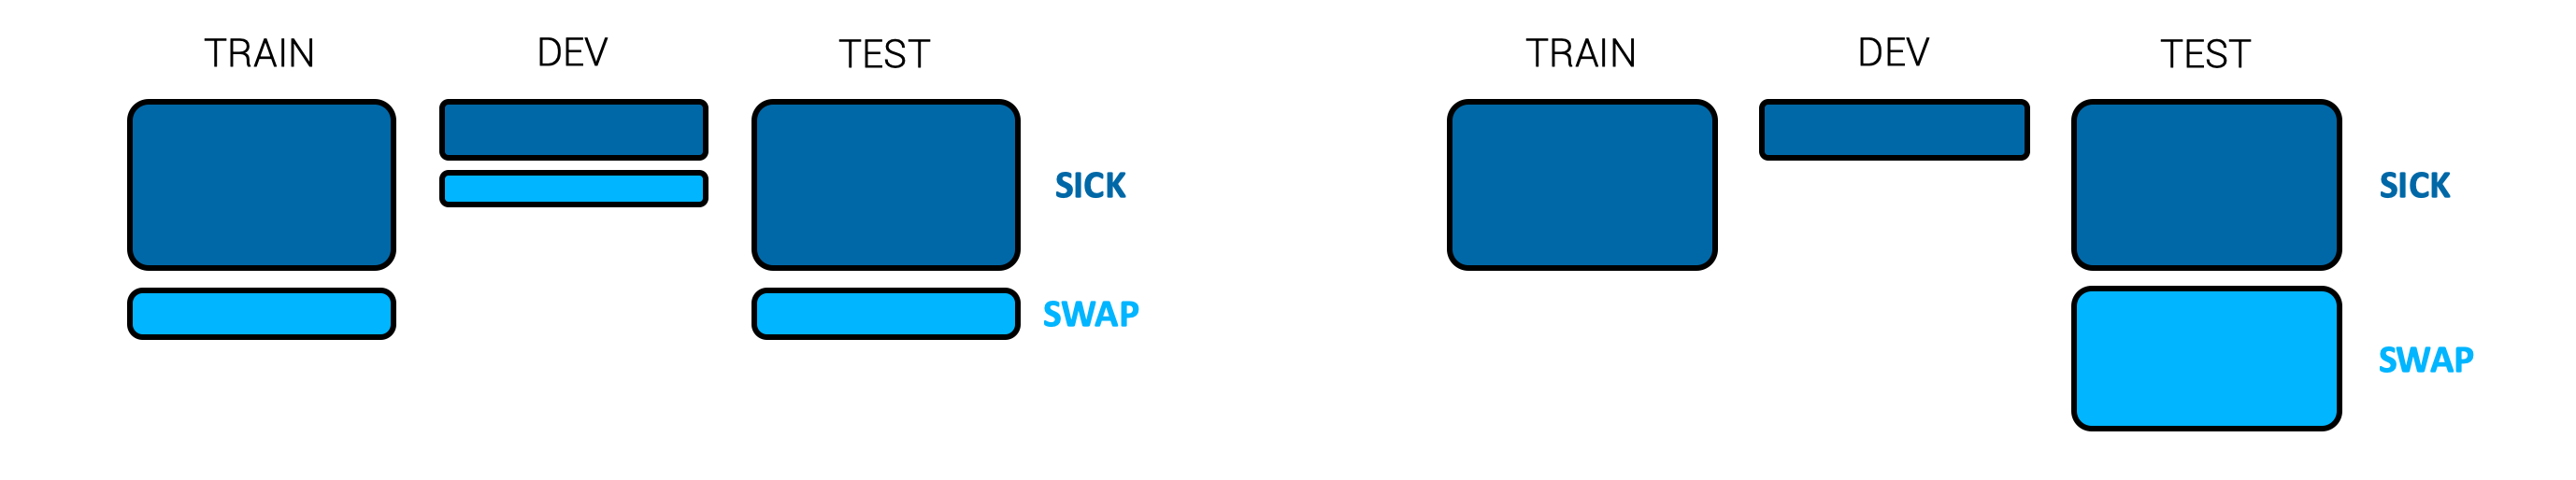
\includegraphics[width=10cm]{images/swap-split.png}
\end{center}
\caption{Concatenation of the dataset: \textit{(right)} we distribute the examples from the SWAP dataset following a stratified train/dev/test split among the corresponding splits of the SICK dataset. \textit{(left)} We only include the SWAP dataset in the SICK test set.}
\labfig{concat}
\end{figure}

As the dataset size is limited, we concatenate the SICK and SWAP datasets. We experiment with two distinct concatenation strategies illustrated in \reffig{concat}. We use a stratified train/dev/test split and distribute the examples among the corresponding split from the SICK dataset. In this configuration, the model is presented with specific examples of the transformation during training. In the second configuration, all examples are included in the SICK test set. During training, the model is not presented with any of the considered examples. Here, we aim to evaluate the ability of the various models to generalize to unseen typologies of examples. Regarding the training setup, we keep the method detailed in Section \ref{sec:training-setup} as well as the hyper-parameters setting.

\subsubsection{Results analysis}

\begin{table*}[!htb]
\footnotesize
% \begin{minipage}{\textwidth}
\centering
\begin{tabularx}{16cm}{@{}l | Y Y Y | Y Y Y@{}}
\toprule
\multirow{2}{*}{} & \multicolumn{3}{c}{\textbf{SWAP}} & \multicolumn{3}{c}{\textbf{SWAP (only SICK training examples)}}\\
 & ALL & SOSWAP & ADAMOD & ALL & SOSWAP & ADAMOD\\\midrule
Test Size & \numprint{6356} & \numprint{485} & \numprint{892} & \numprint{7733} & \numprint{971} & \numprint{1783} \\\midrule
\bow & 72.5 \scriptsize{(1.1)} & 40.7 \scriptsize{(4.1)} & 82.6 \scriptsize{(3.2)} & 53.2 \scriptsize{(4.1)} & \textbf{\underline{16.0}} \scriptsize{(10.4)} & \textbf{\underline{16.5}} \scriptsize{(10.7)}\\
\const & \textbf{85.5} \scriptsize{(0.3)} & \textbf{90.5} \scriptsize{(2.3)} & \textbf{\underline{97.2}} \scriptsize{(1.2)} & 54.3 \scriptsize{(1.1)} & 0.2 \scriptsize{(0.2)} & 6.0 \scriptsize{(3.4)}\\
\seq & 83.7 \scriptsize{(0.9)} & 89.9 \scriptsize{(3.3)} & 95.0 \scriptsize{(1.2)} & 53.5 \scriptsize{(0.3)} & 0.2 \scriptsize{(0.3)} & 0.8 \scriptsize{(0.2)}\\
% \seq (uni) & 81.8 \scriptsize{(2.3)} & 84.1 \scriptsize{(4.5)} & 91.4 \scriptsize{(2.5)} & 54.2 \scriptsize{(1.8)} & 29.7 \scriptsize{(26.9)} & 0.8 \scriptsize{(0.7)}\\
\dep & 84.3 \scriptsize{(0.7)} & 78.4 \scriptsize{(5.1)} & 94.1 \scriptsize{(0.7)} & \textbf{\underline{56.5}} \scriptsize{(0.5)} & 0.3 \scriptsize{(0.4)} & 12.0 \scriptsize{(2.6)}\\\midrule
\bert & \textbf{\underline{86.5}} \scriptsize{(1.6)} & \textbf{\underline{91.4}} \scriptsize{(5.0)} & \textbf{96.6} \scriptsize{(2.1)} & \textbf{53.9} \scriptsize{(0.6)} & \textbf{1.0} \scriptsize{(0.5)} & \textbf{1.0} \scriptsize{(0.7)}\\
\bottomrule
% \toprule
%  & \textbf{null} & \textbf{so} & \textbf{lex} & \textbf{det}\\\midrule
% N & 2787 & 473 & 407 & 121\\\midrule
% Dependency & 85,15 & \textbf{72,73} & 70,52 & 99,17\\
% Constituency & 84,18 & 68,5 & 72,97 & 97,52\\
% Sequence (BERT) & \textbf{87,94} & 64,48 & \textbf{79,85} & \textbf{100,00}\\
% Sequence (GRU) & 84,61 & 70,4 & 72,48 & \textbf{100,00}\\
% Bag Of Words & 82,63 & 52,01 & 55,04 & 81,82\\
% \bottomrule
\end{tabularx}
\caption{Accuracy on the test set for SICK-E and SWAP task given the two proposed aggregation strategies. We report a mean over 5 runs (standard deviations in parentheses). The best results for a given embedding are in \textbf{bold}. The best results overall are \underline{underlined}.}
\label{table:focus-swap}
\end{table*}

We present the accuracy scores on the test set in Table \ref{table:focus-swap}. In the two concatenation strategies, we present the accuracy of the entire test set and filter on the SOSWAP and ADAMOD test pairs. 

The transformations in the SWAP dataset are much more limited than in the SICK dataset which includes additional transformations such as verb transitive/intransitive alternations or exploiting homonymy and polysemy. 
Nevertheless, when no example is included in the training set, the accuracy scores seem in line with the one for the words scrambling \textbf{(ws)} transformation for the SICK dataset in Table \ref{table:transformation-global}. 

For both transformations, all models fail to predict the correct label when not exposed to the transformation during the training. Only the \bow model stands out but with a substantial standard variation. However, the \dep model seems not entirely tricked by the ADAMOD transformation. Even more remarkable, \bert is completely fooled as well. From these specific swapping examples, we assume that despite explicit structure assimilation in the model, they may not be able to generalize to a specific topology of unseen examples. This may also contribute to the lower results for the words scrambling \textbf{(ws)} on the SICK task.

% \FloatBarrier
% \subsection{PAWS dataset}

% The PAWS \parencite{zhang_19} contains 108,463 human-labeled labeled pairs that feature the importance of modeling structure, context, and word order information for the problem of paraphrase identification. The dataset has two subsets, one based on Wikipedia and the other one based on the Quora Question Pairs (QQP) dataset. 

% We split the dataset using a 


% \begin{table}[!htb]
% \footnotesize
% % \begin{minipage}{\textwidth}

% \centering {
% \begin{tabularx}{\columnwidth}{@{}Y Y Y Y Y Y@{}}
% \toprule
%  & \bow & \const & \seq & \dep & \bert \\\midrule
% \textbf{PAWS} & 67.6 \scriptsize{(0.3)} & 82.7 \scriptsize{(0.1)} & 83.6 % \scriptsize{(0.2)}  & 75.7 \scriptsize{(0.2)} & \textit{90.1} \\
% \bottomrule
% % \toprule
% %  & \textbf{null} & \textbf{so} & \textbf{lex} & \textbf{det}\\\midrule
% % N & 2787 & 473 & 407 & 121\\\midrule
% % Dependency & 85,15 & \textbf{72,73} & 70,52 & 99,17\\
% % Constituency & 84,18 & 68,5 & 72,97 & 97,52\\
% % Sequence (BERT) & \textbf{87,94} & 64,48 & \textbf{79,85} & \textbf{100,00}\\
% % Sequence (GRU) & 84,61 & 70,4 & 72,48 & \textbf{100,00}\\
% % Bag Of Words & 82,63 & 52,01 & 55,04 & 81,82\\
% % \bottomrule
% \end{tabularx}}
% \caption{Accuracy on the test set for SICK-E task for pair samples with lexical transformations. We report mean over 5 runs (standard deviations in parentheses). Best results for a given embedding are in \textbf{bold}. Best results overall are \underline{underlined}.}
% \label{table:paws}
% \end{table}


%%%%%%%%%%%%%%%%%%%%%%%%%%%%%%%%%%%%%%%%%%%%%%%%%%%%%%%%%%%%%%%%%%%%%%%%%%%%%
% \subsection{Conclusion and future work}

% We conducted experiment to evaluate the ability of models to perform compositional knowledge in a natural language inference task. More specifically we quantified, for each model, its robustness toward specific linguistic structures. The heterogeneity of results suggests that models do capture distinct types of information. Moreover, pre-trained \bert models seem to encode additional information not captured by others. Indeed, models using \bert embeddings almost systematically achieve a better score. 

% However, cases remain for which structured models can improve the performance of stand-alone contextualized embeddings. In such cases, syntactic information may not be fully encoded in \bert. We identified a specific transformation which consist in replacing word with semantic opposite. For such transformation, \bert contextualized embeddings leads to surprisingly low performances.

% Finally, we identified cases for which all models fail, in particular for the word scrambling transformation. We proposed an experimental setup to focus more precisely on the later and observe that some subcases could, to some extend, be addressed by balancing the training set distribution. However, for such complex linguistic structures, we observe a room for improvement to capture the compositional structure and common sense knowledge within NLP models.

%%%%%%%%%%%%%%%%%%%%%%%%%%%%%%%%%%%%%%%%%%%%%%%%%%%%%%%%%%%%%%%%%%%%%%%%%%%%%%%%%%%%%%%%%%%%%%%%%%%%%%%%%%%%%%%%%%%%%%%%%%%%%%%%%%%%%%%%%%%%%%%%%%%%%%

\section{Arithmetic expressions evaluation}
\labsec{composition:arithmetic}

% \bcomment{Missing transition}{what is the problem you address here ? how does it relate to the previous one ?}

% Evaluating model compositional properties is notoriously hard. First—as for every other language evaluation benchmark—creating the data is a critical step. Labeling raw data is time-consuming and it is difficult to control precisely the property of the examples. On the other hand, generating artificial data may lead to poor lexical or structural diversity. Additionally, studies show that models might use lexical biases or shallow heuristics in the data to achieve the task \cite{linzen_18}. Popular benchmarks require to generate the answer, which makes it difficult to disentangle the effect of the encoding and decoding parts. Indeed,  some errors might be related to the decoding part. This makes it difficult to precisely assess model compositional properties. 

So far, we used data generated via a semi-automated procedure, which enables precise control of the property of the examples. On the other hand, generating artificial data may lead to poor lexical or structural diversity. Studies show that models might use lexical biases or shallow heuristics in the data to achieve the task \parencite{linzen_18}. Consequently, shallow lexical and structural pattern matching operations may be difficult to distinguish from effective compositional operations.

Here, we aim to examine the compositional properties of neural architectures without being affected by lexical phenomena. Therefore, we propose a setup for which neural models compose representations for sentences that do not include words: arithmetic expressions. Arithmetic defines a self-contained universe which can be described using a limited set of symbols and composition rules. This makes it easy to build specific examples with isolated properties. By extension, we may evaluate neural model compositional abilities. Indeed, numerically evaluating formal expressions theoretically requires capturing the formal rules of arithmetic. We use the work from \textcite{hupkes_20} and consider aspects of compositionality that may also be declined for language: localism, substitutivity, productivity, and systematicity.

Neural networks may be properly trained to solve mathematical expressions. A line of work outlines that pre-trained language models or static word embeddings capture scales and notions of numeracy \parencite{wallace_19, naik_19, sundararaman_20, zhang_20, thawani_21}. Beyond representing numbers, further work also analyzes the ability of models to perform basic mathematics reasoning \parencite{saxton_19, dua_19, geva_20} or solve mathematical expressions \parencite{lample_20}.

Many of these related works mix raw text and numeracy and focus on the ability of language models to handle numeric representations. However, our problem is different. Therefore, we introduce \textbf{CobA}, a \textbf{Co}mpositionality \textbf{b}enchmark using \textbf{A}rithmetic. The dataset consists of simple arithmetic expressions combining natural integers with addition and multiplication operators. For example, $(5 + 4) \times 2$. We generate partitions of the dataset with specific in-domain and generalization sets, designed to evaluate the model's ability for each compositional aspect: localism, substitutivity, productivity, and systematicity. 


% The key contribution in our work is to build a dataset of arithmetic expressions to evaluate neural model compositional abilities. Indeed, numerically evaluating formal expressions theoretically requires capturing the formal rules of arithmetic. CobA focuses on aspects of compositionality that may also be declined for language \parencite{hupkes_20}. But contrary to previous work, we do not mix raw text and numeracy. We derive many arithmetic expressions, using limited formal explicit rules and symbols. In this section, we detail the generation of the dataset.

% \bcomment{In this section, we introduce \textbf{CobA}, a \textbf{Co}mpositionality \textbf{b}enchmark using \textbf{A}rithmetic. The dataset consists of simple arithmetic expressions combining natural integers with addition and multiplication operators. For example, $(5 + 4) \times 2$. We distinguish four aspects of compositionality: localism, substitutivity, productivity, and systematicity. We generate partitions of the dataset with specific in-domain and generalization sets, designed to evaluate the model's ability for each compositional aspect. By carefully selecting expressions from the in-domain and generalization sets, we introduce controlled differences between the two sets.  We show that models achieve competitive performance on a random partition, for which there is no controlled difference. Yet, for partitions requiring compositional extrapolation, performances drastically decrease for most encoder architectures.}{to rewrite, its too mixed ; first the problem and the motivations, then the method and the dataset }


% Moreover, we formulate the benchmark as a classification task. The task can be solved using a simple encoder, without the need to decode the answer. Thus, our setup minimizes complex interactions between encoding and decoding.
%and indecipherable 

In \refsec{composition:arithmetic:method}, we detail the data generation process and the distinct dataset partitions. In \refsec{composition:arithmetic:method}, we present our training and evaluation setup. We also present our main results on the CobA generalization set. In \refsec{composition:arithmetic:ablation-study}, we perform an in-depth study to analyze better how the choice of hyper-parameters might leverage specific performances and how the expression complexity impacts model performances.

% \bcomment{problem of strcuture}{we do not know what is sytematicity etc. First state your problem and describe these 4 properties then describe the dataset. The current mix in the chapter is problematic}


\subsection{Dataset description}
\labsec{composition:arithmetic:method}


% \begin{figure*}[htb!]
%     \centering
%     \includegraphics[width=\textwidth]{figures/stats_2.png}
%     \caption{Dataset distributions given partitions}
%     \label{fig:stats}
% \end{figure*}

\subsubsection{Generation procedure}

Using an automatic procedure, we generate arithmetic expressions. First, we generate a natural integer between 1 and 100, for example, $34$. We then decompose it into the addition or multiplication of two other integers, such as $2 \times 17$. We then recursively decompose each integer in the new expression as the product or sum of two integers or keep it unchanged, with a probability $p$\sidenote{We implement specific rules for numbers that are prime and cannot be decomposed with multiplication. We set the probability $p$ to expand, by default, at $0.5$.}.

% \begin{algorithm}
% \caption{Expand expressions}\label{alg:expression-generation}
% $E \gets e$\; 
% $P_{\times} \gets p_{\times}$\;
% $P_{+} \gets p_{+}$\;
% \For{$N \in E$}{
%   \eIf{$P_{\times} \ge p_{floor}$ and $N$ is not prime}{
%     $N \gets N_1 \times N_2$\;
%     $E \gets expand(N_1) \times expand(N_2)$\;
%   }{\If{$P_{+} \ge p_{floor}$}{
%       $N \gets N_1 + N_2$\;
%       $E \gets expand(N_1) + expand(N_2)$\;
%     }
%   }
% }
% \end{algorithm}

As in \textcite{lample_20}, we use prefix notation (also known as normal Polish notation). The arithmetic expression $2 \times (14 + 3)$ is represented as the sequence $\times 2 + 14 \: 3$. This notation avoids the use of parenthesis and therefore leads to shorter expressions. We assign each symbol—natural integer or operator sign—to a given token. We distinguish between two distinct left and right-hand sides of an operator for each expression. For example, we make the distinction between the expression $14 + 3$ and $3 + 14$. We generate over 2.5M unique expressions with between 0 and 9 operators given this procedure.

\begin{table*}[t]
    \footnotesize
    \begin{tabularx}{16cm}{X|ccccc}
    % \begin{tabular}{lccccccccc}
    \toprule
    \textbf{Partitions} & \textbf{Random} & \textbf{Systematicity} & \textbf{Productivity} & \textbf{Localism} & \textbf{Substitutivity} \\
    % \hline
    \midrule
    Mean value & 66.3 / 66.2 & 67.0 / 68.2 & 66.4 / 65.3 & 66.1 / 67.4 & 66.1 / 66.4 \\
    Min number of operators & 0 / 0 & 2 / 2 & \textbf{0 / 4} & 2 / 2 & 2 / 2 \\
    Mean number of operators & 2.8 / 2.8 & 2.6 / 2.5 & \textbf{2.8 / 6.5} & 2.8 / 2.7 & 2.8 / 2.7 \\
    Max number of operators & 3 / 3 & 3 / 3 & \textbf{3 / 9} & 3 / 3 & 3 / 3 \\
    \addlinespace
    Expressions with odds and evens (\%) & 85.6 / 85.4 & \textbf{0.0 / 100.0} & 85.6 / 98.3 & 85.7 / 85.3 & 85.7 / 85.1 \\
    Swapped-expressions in-domain (\%) & 1.3 / 1.6 & 10.0 / 0.0 & 1.2 / 0.0 & 1.2 / 1.5 & \textbf{0.0 / 0.0} \\
    Sub-expressions in-domain (\%) & 2.2 / 2.3 & 4.2 / 1.3 & 2.1 / 0.7 & \textbf{0.0 / 00} & 1.0 / 1.1 \\
    % \addlinespace
    \bottomrule
    \end{tabularx}
    \caption{Key statistics given each partition of the dataset. We report the figures for the in-domain / generalization set for each statistic. We express the "Expressions with odds and evens", "Swapped-expressions in-domain" and "sub-expressions in-domain" as the proportion of expressions verifying the property for each set. The statistics that are determinants for the aspect studied in a given partition appear in \textbf{bold}.}
    \label{table:paritions}
\end{table*}


\subsubsection{Partitioning the dataset}
\label{subsec:partition}

% random	localism	systematicity	productivity	substitutivity
% random	[39.4, 0.1]	[60.3, 0.1]	[39.9, 0.1]	[39.2, 0.1]	[59.7, 0.2]
% bow	[35.9, 9.9]	[22.5, 12.3]	[36.2, 1.8]	[37.5, 3.1]	[0.0, 0.0]
% rnn	[2.3, 0.5]	[8.9, 0.9]	[2.3, 0.3]	[13.7, 0.8]	[2.6, 0.2]
% bi_rnn	[1.5, 0.2]	[9.5, 0.6]	[2.1, 0.4]	[11.8, 1.3]	[2.3, 0.4]
% tree_rnn	[4.7, 0.2]	[10.9, 0.2]	[5.9, 0.2]	[16.1, 1.1]	[6.0, 0.2]
% albert	[4.4, 0.7]	[7.8, 8.0]	[16.9, 0.0]	[25.8, 0.1]	[5.0, 0.3]
% transformer	[3.0, 0.6]	[14.0, 0.0]	[11.9, 2.7]	[28.0, 1.5]	[3.1, 0.9]

Our dataset aims at evaluating model compositional properties. We take inspiration from the procedure proposed in SCAN \parencite{lake_18, loula_18}. We carefully select expressions to create partitions (in-domain and generalization sets) from the dataset. We split them such that in-domain and generalization sets have different distributions. It is impossible to infer generalization examples without fully capturing the properties ruling this specific aspect in the in-domain set. We thus compare the ability of models to perform \textit{out-of-domain} generalization. We distinguish between model learning shallow heuristics such as local pattern matching and the one learning true compositional operations.

% \bcomment{comes too late}{...}
We build partitions given the work from \textcite{hupkes_20}, which distinguishes sub-properties within compositionality. \textbf{Localism}, \textbf{Substitutivity}, \textbf{Productivity} and \textbf{Systematicity}\sidenote{\textcite{hupkes_20} also enumerate the over-generalisation aspect which evaluate the accommodation to exceptions. However, we find it complex to adapt this property for our specific dataset and therefore discard it in this work.}. Each of the partitions detailed below has a key statistic distribution and is designed to evaluate a model's performance along a given aspect. Each partition contains an in-domain set of 24,000 expressions and a generalization set of 12,000 expressions. We present other key statistics for the partitions in Table~\ref{table:paritions}. 

\begin{figure}[htb!]
    \centering
    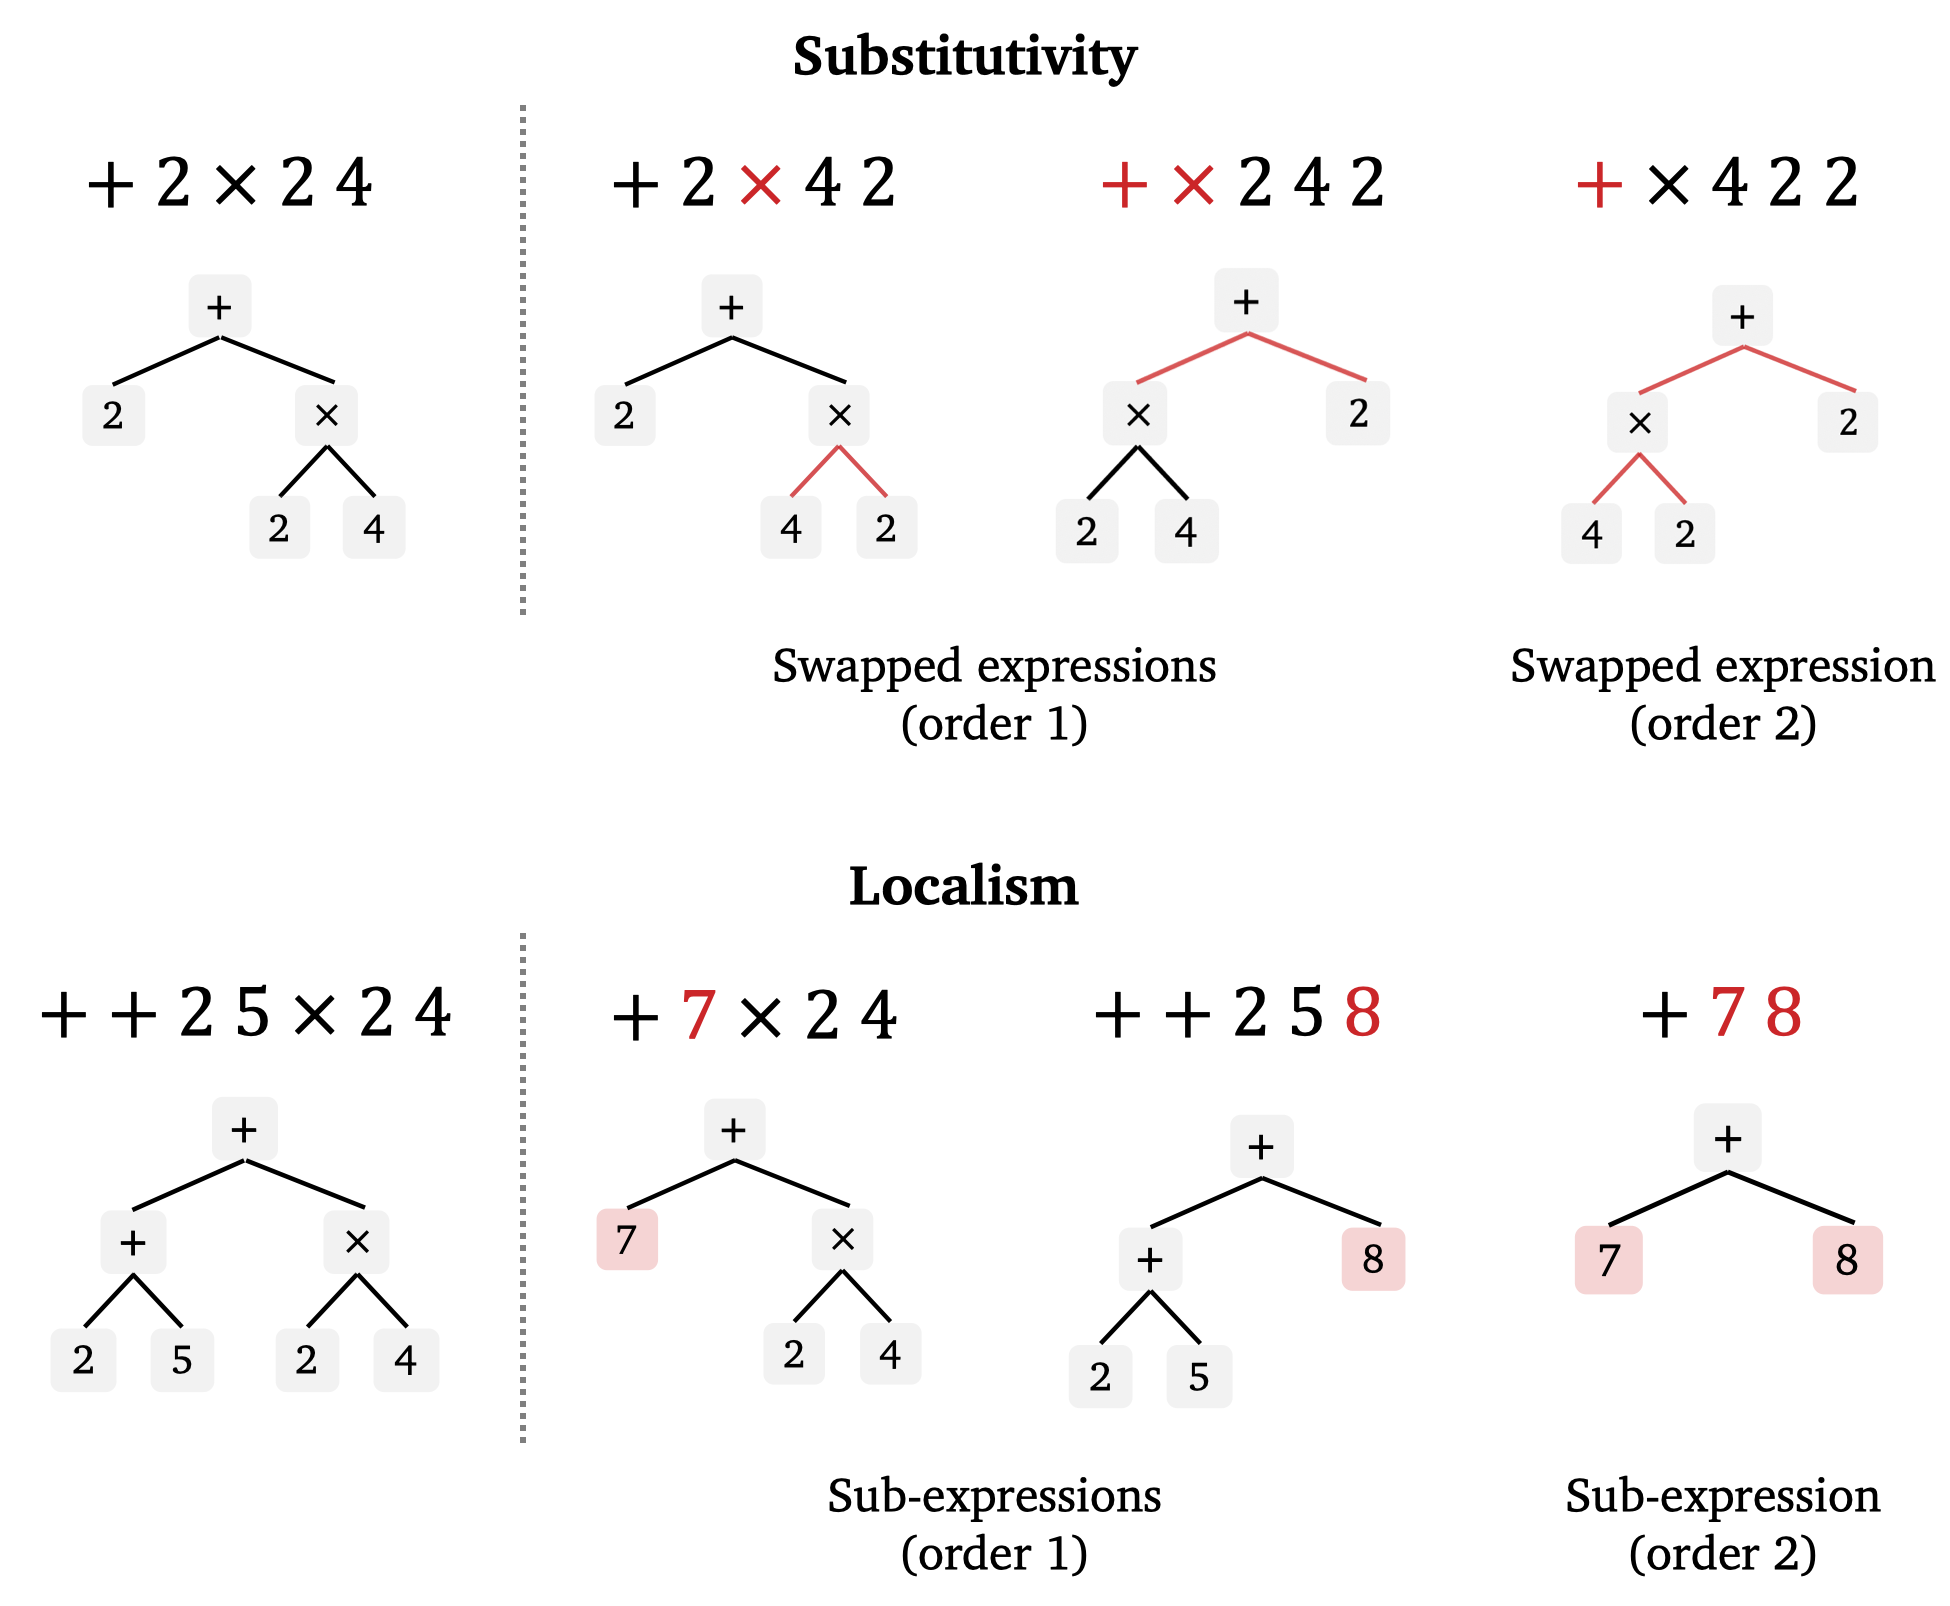
\includegraphics[width=\textwidth]{images/loc_prod_6.png}
    \caption{Generation of expressions tuples for probing substitutivity and localism. For localism, we can deduce expressions from the expression seed by evaluating sub-components. For substitutivity, we can deduce expressions from each other by swapping operators' left and right-hand sides. For the clarity of the illustration, we use the infix form for the expressions.}
    \labfig{loc_prod}
\end{figure}

% Each aspect evaluates a specific ability: \textbf{Localism} the recursive evaluation of smaller constituents before larger constituents \textbf{Substitutivity} the robustness towards the introduction of synonyms \textbf{Productivity} the extrapolation to longer sequences \textbf{Systematicity} the recombination of known parts to form new sequences

% This procedure is inspired by the one used for the SCAN task \parencite{lake_18, loula_18}. The dataset is split using a \textit{random} partition for which train and test examples are distinct but without any specific control. Other partitions evaluate systematicity, since they contain sub-parts in isolation in the training set and recombined with other in the test set. We use the distinction made from \textcite{hupkes_20} to provide a fine-grained analysis. For each sub-property, we generate a partition with specific training and testing distribution design to assess the model ability for this specific aspect. These partitions are detailed below.

\paragraph{Random} is a regular training procedure. We split the dataset randomly without any specific control during the selection of the expressions. While in-domain and generalization examples are all distinct, they share the same distributions and have similar underlying characteristics.

\paragraph{Systematicity} evaluates the recombination of known parts to form new sequences. We build the partition using the distinction between odd and even natural integers. The training set contains expressions with either only odd or even numbers. For examples $2 \times 4 + 8$. or $3 + 5 + 7$. The test set contains expressions with both even and odd numbers such as $3 + 2 \times 5 + 4$.

\paragraph{Productivity} evaluates the extrapolation to longer sequences. We train the model on expression with up to 3 operators. We then evaluate the model on longer expressions with up to 9 operators.

% For the localism and substitutivity partitions, We structure the generalization set by pairing expressions. For the localism partition, we pair each expression with the same expression whose intermediate values have been computed. For the substitutivity partition, we pair each expression with an expression for which we swapped the left and right sides of some operators. We give an illustration in Figure~\ref{fig:loc_prod}.

\paragraph{Substitutivity} evaluates the robustness towards the introduction of synonyms. In our work, we interpret this definition as the robustness towards paraphrases and evaluate the ability of models to perceive an operator's commutative property. We organize our dataset as a collection of "swapped expressions". Swapped expressions are tuples of expressions with the same value and only differ by swapping each operator's left and right-hand sides. We illustrate this swapping organization in \reffig{loc_prod}. During training, we only expose the model to a single expression per tuple. Therefore the model cannot learn the commutative property from shallow pattern matching. During the evaluation, we evaluate the model's commutative ability by comparing couples of predicted values for expressions from the same tuple.
% \bcomment{provide an example}{figure on top?}

% as illustrated in Figure~\ref{fig:loc_prod}, we include in the generalization set expressions for which the left and right-hand sides of one or multiple operators have been switched. We evaluate the encoder robustness towards these swaps by comparing the gap between the evaluation of the two swapped expressions.

\paragraph{Localism} evaluates the recursive evaluation of smaller constituents before larger constituents. We also organize our dataset as a collection of "sub-expressions". Sub expressions are tuples of expressions with the same value that only differ by the level of decomposition of the expressions as illustrated in \reffig{loc_prod}. We use the same training and evaluation protocol as for Substitutivity.

% \bccomment{to remove (redundant stuff) : evaluating intermediate operators. We illustrate this organization in Figure~\ref{fig:loc_prod}. During training, we only expose the model to one expression per tuple. During evaluation, we compare two predicted value for expressions from the same tuple. We aim to assess whether the model recursively evaluate the local sub-components or rely on general heuristic to process the expression.}

% To assess this ability, we compare the evaluation of a given expression and the same expression for which one or multiple sub-components have been evaluated. As illustrated in Figure~\ref{fig:loc_prod}, we compare for example, the evaluation of the expression $2 + 5 + 2 \times 4$ and $7 + 2 \times 4$. By measuring the gap between these two evaluations, we aim to assess whether the model evaluate the local sub-component $2 + 5$ or rely on general heuristic to process the expression.

\subsection{Experiments}
\labsec{composition:arithmetic:experiments}

\begin{figure*}[htb!]
    \centering
    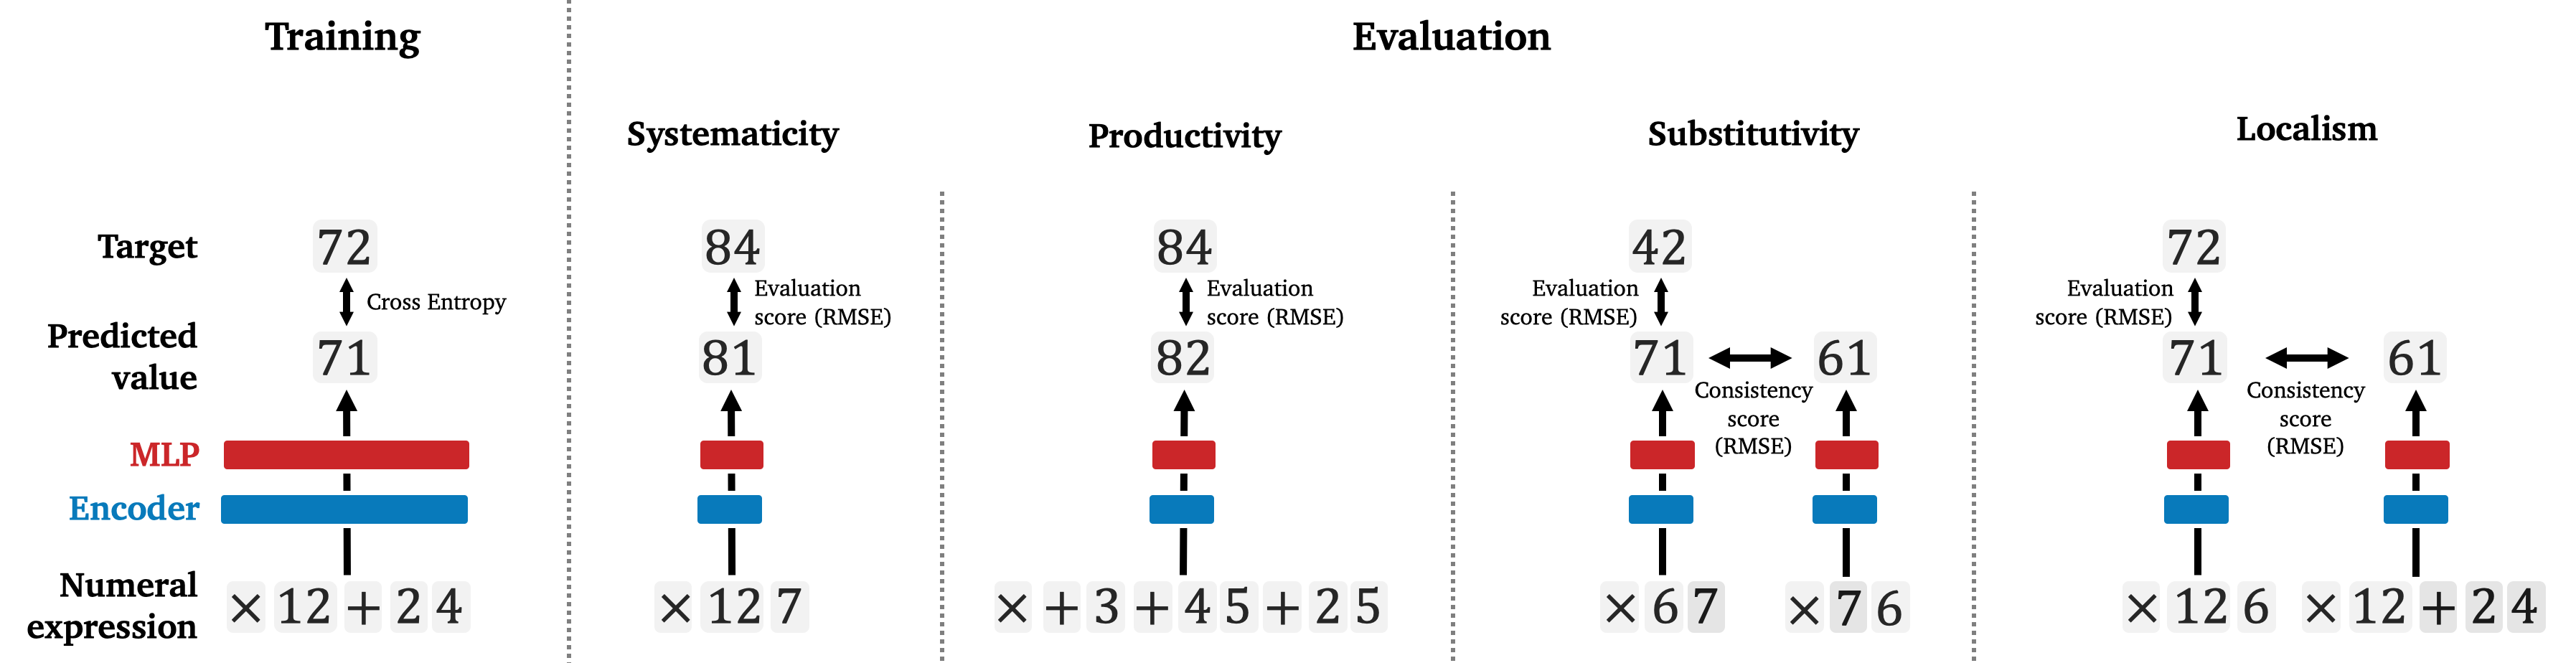
\includegraphics[width=16cm]{images/compositional_tasks_5.png}
    \caption{Illustration of the train and evaluation setup for assessing model compositional properties using the CobA dataset. We train the model to evaluate in-domain expressions. We then infer expressions from the generalization set. The dataset includes partitions for \textbf{Localism}, \textbf{Substitutivity}, \textbf{Productivity}, and \textbf{Systematicity}.}
    \label{fig:illustration}
\end{figure*}

% \sidenotetext{The RMSE harmonic mean assesses the consistency of the model prediction between two expressions pair as well as the general consistency of the model. It for example allows to discard trivial models which always predict the same value}

We train the model using a classification objective. Given an arithmetic expression, the model predicts its value among the 100 possible integers. This setup avoids using a complex decoder module~;  a simple probe is sufficient. The architecture is decomposed as follows: first, an encoder maps the arithmetic expression to an embedding vector. Then, a two-layer perceptron followed by a softmax outputs a probability distribution. We train the model by minimizing a cross-entropy loss.

\subsubsection{Encoder architectures}

As in \refsec{composition:nli}, we use BoW, sequential LSTM, N-ary tree LSTM. We also consider transformer architectures. We derive two simple encoders from the architectures of \textsc{Bert} \parencite{devlin_19} and \textsc{Albert} \parencite{lan_20}. We use the \textsc{[CLS]} token hidden state from the last layer as expression embedding. We initialize our models randomly and train them from scratch. Their architectures are light compared with standard transformer scales: we use a hidden size of 128, 6 hidden layers, and 8 attention heads. This represents 1.2M parameters for \textsc{Bert} and 300k for \textsc{Albert} since parameters are tied across layers. As observed in \textcite{csordas_21} and \textcite{onta_21}, transformers' positional encoding are particularly important for this task. We use the method from \textcite{wallace_19} and add some random padding at the beginning of the input so that the encoder does not solve the task by overfitting the absolute position of the symbols.



% We discuss the effect of such configuration in Section~\ref{subsec:positional-embeddings}.

\subsubsection{Training configuration}

We design all encoders comparable, with roughly the same number of parameters (1.2M), as detailed in Table~\ref{table:results-main}. We also use the same hidden and embedding size range for all encoders: 256 for LSTM-based encoders and 128 for transformer-based encoders. We use the same optimization procedure for each model.
%and verify that they all reach the same level of convergence on a development test. 
We train all models using the AdamW optimizer \parencite{loshchilov_19} with a $1e^{-3}$ learning rate, 1 epoch warm-up with polynomial decay and a batch size of 100. For each partition, we separate the in-domain set between a train and dev set using a random 90/10\% split. We measure the RMSE between the expression predicted and the true value on the dev set. We stop the training when no improvement is made for 5 consecutive epochs or after 100 maximum epochs\sidenote{For some runs, we observed that the initialization of the model weights prevented any decrease of the loss. In such cases, we immediately stopped the run and relaunched it with a new random seed.}. We train all models on an Nvidia 2080 Ti GPU. The training time is around 10 minutes per partition and model. We set parameters given the literature on the subject and do not perform hyper-parameters search.

% \bcomment{It remains to get embeddings for natural numbers...}{}
Regarding the natural integer embeddings, we use the DICE method \parencite{sundararaman_20}. The method uses a deterministic approach to construct natural integer embeddings. It obtains state-of-the-art results on evaluation benchmarks \parencite{wallace_19}. We do not update natural integer embeddings during training. For operators and specific tokens such as CLS or SEP tokens, we initialize embeddings randomly (with the same scale) and update them during training. 
% We challenge the use of this initialization method in Section~\ref{subsec:embeddings}

\subsubsection{Evaluation setup}

\begin{table*}[t]
    \footnotesize
    \begin{tabularx}{16cm}{lY|ccccc}
    % \begin{tabular}{lccccccccc}
    \toprule
    \textbf{Encoders} & \textbf{\# parameters} ($\times 1e^3$) & \textbf{Random} & \textbf{Localism} & \textbf{Systematicity} & \textbf{Productivity} & \textbf{Substitutivity} \\
    % \hline
    \midrule
    Random & --- & 39.5 {\scriptsize (0.1)} & 40.1 {\scriptsize (0.1)} & 40.0  {\scriptsize (0.2)} & 39.1 {\scriptsize (0.2)} & 40.0 {\scriptsize (0.2)} \\
    BoW & 68 & 28.7 {\scriptsize (8.1)} & 20.6 {\scriptsize (4.8)} & 37.0 {\scriptsize (0.2)} & 38.3 {\scriptsize (5.4)} & 19.0 {\scriptsize (0.5)} \\
    \addlinespace
    \textsc{LSTM} (uni) & 595 & 3.5 {\scriptsize (0.4)} & 7.3 {\scriptsize (0.8)} & 2.7 {\scriptsize (0.3)} & 14.1 {\scriptsize (0.4)} & 2.4 {\scriptsize (0.3)} \\
    \textsc{LSTM} (bi) & \numprint{1186} & 2.2 {\scriptsize (0.2)} & 8.6 {\scriptsize (1.0)} & 2.5 {\scriptsize (0.3)} & 13.5 {\scriptsize (1.1)} & 1.3 {\scriptsize (0.1)} \\
    \textsc{LSTM} (tree) & \numprint{1012} & 5.4 {\scriptsize (0.1)} & 8.9 {\scriptsize (0.1)} & 7.4 {\scriptsize (0.6)} & 15.0 {\scriptsize (0.5)} & 4.9 {\scriptsize (0.3)} \\
    \addlinespace
    Transformer (\textsc{Bert}) & \numprint{1290} & 3.6 {\scriptsize (1.1)} & 11.9 {\scriptsize (0.7)} &  20.6 {\scriptsize (4.9)} & 30.2 {\scriptsize (1.8)} &	2.3 {\scriptsize (0.8)} \\
    Transformer (\textsc{Albert}) & 315 & 6.9 {\scriptsize (1.5)} & 13.0 {\scriptsize (0.9)} & 16.6 {\scriptsize (6.6)} & 25.9 {\scriptsize (3.1)} &	 4.8 {\scriptsize (1.0)} \\
    % \addlinespace
    \bottomrule
    \end{tabularx}
    \caption{Compositionality evaluation. We report metrics from the generalization set. For the random, systematicity and productivity partitions, we report the evaluation score, which is the RMSE between the true and the predicted values. For the localism and substitutivity partitions, we report the mean between the evaluation and consistency score. For each metric, we report the mean value over 4 runs (standard deviation in parentheses).} % \protect\footnotemark.
    % We report the harmonic mean between the two metrics.
    % We compute it as the harmonic mean between \textit{(i)} the RMSE between the expression true and predicted value and \textit{(ii)} the RMSE between the expression predicted value and a paired expression predicted value.
    \label{table:results-main}
\end{table*}

% \begin{table*}[t]
%     \footnotesize
%     \begin{tabularx}{\textwidth}{lY|YYYYY}
%     % \begin{tabular}{lccccccccc}
%     \toprule
%     \textbf{Encoders} & \textbf{Number of parameters} ($\times 100$) & \textbf{Random} & \textbf{Localism} & \textbf{Systematicity} & \textbf{Productivity} & \textbf{Substitutivity} \\
%     % \hline
%     \midrule
%     Random & --- & 39.4 {\scriptsize (0.1)} & 40.1 {\scriptsize (0.1)} & 39.9  {\scriptsize (0.1)} & 39.2 {\scriptsize (0.1)} & 39.9 {\scriptsize (0.2)} \\
%     BoW & 68 & 35.9 {\scriptsize (9.9)} & 15.0 {\scriptsize (8.2)} & 36.2 {\scriptsize (1.8)} & 37.5 {\scriptsize (3.1)} & 0.0 {\scriptsize (0.0)} \\
%     \addlinespace
%     \textsc{LSTM} (uni) & 595 & 2.3 {\scriptsize (0.5)} & 5.9 {\scriptsize (0.6)} & 2.3 {\scriptsize (0.3)} & 13.7 {\scriptsize (0.8)} & 1.7 {\scriptsize (0.2)} \\
%     \textsc{LSTM} (bi) & 1,186 & 1.5 {\scriptsize (0.2)} & 6.3 {\scriptsize (0.4)} & 2.1 {\scriptsize (0.4)} & 11.8 {\scriptsize (1.3)} & 1.5 {\scriptsize (0.3)} \\
%     \textsc{LSTM} (tree) & 1,012 & 4.7 {\scriptsize (0.2)} & 7.3 {\scriptsize (0.2)} & 5.9 {\scriptsize (0.2)} & 16.1 {\scriptsize (1.1)} & 4.0 {\scriptsize (0.1)} \\
%     \addlinespace
%     Transformer (\textsc{Bert}) & 1,290 & 4.4 {\scriptsize (0.7)} & 9.3 {\scriptsize (0.0)} &  16.9 {\scriptsize (0.0)} & 25.8 {\scriptsize (0.1)} &	2.1 {\scriptsize (0.6)} \\
%     Transformer (\textsc{Albert}) & 315 & 3.0 {\scriptsize (0.6)} & 5.2 {\scriptsize (5.3)} & 11.9 {\scriptsize (2.7)} & 28.0 {\scriptsize (1.5)} &	 3.3 {\scriptsize (0.2)} \\
%     % \addlinespace
%     \bottomrule
%     \end{tabularx}
%     \caption{Compositionality evaluation. We report metrics from the generalization set. For the random, systematicity and productivity partitions, we report the evaluation score, which is the RMSE between the true and the predicted values. For the localism and ssubstitutivity partitions, we report the harmonic mean between the evaluation and consistency score. For each metric, we report the mean value over 5 runs (standard deviation in parentheses).} % \protect\footnotemark.
%     % We report the harmonic mean between the two metrics.
%     % We compute it as the harmonic mean between \textit{(i)} the RMSE between the expression true and predicted value and \textit{(ii)} the RMSE between the expression predicted value and a paired expression predicted value.
%     \label{table:results-main}
% \end{table*}

We evaluate our models and report metrics from the generalization set. We illustrate the evaluation setup in Figure~\ref{fig:illustration}. For the random, systematicity, and productivity partitions, we compute an evaluation score as the mean RMSE\sidenote{The root-mean-square error (RMSE) between a predicted vector $\hat{y}$ and a reference $y$ of dimensions $n$ is defined as $RMSE(\hat{y}, y) = \sqrt{\sum_{i=1}^{n}\frac{\left(\hat{y}_i - y_i\right)^2}{n}}$.} between each expression's true and predicted value. For the localism and substitutivity partitions, we refine the evaluation procedure to take advantage of the additional paired structure of the partition described in section \ref{subsec:partition}. We compute both an \textit{agreement} score as the mean RMSE between the predicted values from the two expressions of each pair and an \textit{evaluation} score as the RMSE between the predicted and true value of the expression. We report the mean between the \textit{agreement} and \textit{evaluation} scores. This score reflects the consistency of the model's predictions between two expressions as well as its ability to predict the true value. It, for example, discards trivial models which always predict the same value or model accurately evaluating one expression of the pair but failing for the other.

% \bccomment{remove this : We structure the generalization set by pairing expressions. For the localism partition, we pair each expression with the same expression whose intermediate values have been computed. For the substitutivity partition, we pair each expression with an expression for which we swapped the left and right sides of some operators. We give an illustration in Figure~\ref{fig:loc_prod}. }

\subsubsection{Results}
\label{sec:results}

% \begin{figure*}[htb!]
%     \centering
%     \includegraphics[width=\textwidth]{figures/productivity.png}
%     \caption{Evolution of the RMSE test given the number of operators.}
%     \label{fig:productivity}
% \end{figure*}

Table~\ref{table:results-main} presents the results on the generalization set. We use two baselines: one that randomly predicts the value of any expression and the BoW model. We use the RMSE to compare the models. The lower it is, the better are predictions on average.

By a small margin, BoW outperforms the random guessing baseline. This suggests that the task requires accounting for the expression structure. Lexical information may provide insights for solving the task: an expression containing numbers such as a $56$ and $43$ is more likely of being equal to a high value such as $89$ than an expression containing only a $2$ and a $3$. Yet, local information alone may not be sufficient to solve the task since expressions with a high overlap may greatly differ in value. For example, the expressions $3+3$ and $3\times3$ contain the same symbols but are not equal since they used different mathematical operators. 
Models can generalize to examples with similar distributions. On the random partition, all the models indeed achieve low RMSE, significantly lower than the baselines. Models are also robust toward the introduction of paraphrases since scores on substitutivity and random partitions are similar. For other partitions, results are more contrasted.

In general, encoders relying on LSTM cells outperform transformers. For productivity and systematicity, sequential models strongly outperform models using fixed-length context. Surprisingly, sequential LSTMs constantly outperform tree LSTMs, despite having fewer structural biases.

Regarding transformers, the RMSE highly deteriorates for productivity. We confirm their known limitation in terms of productivity. We also observe transformers stumbling upon systematicity. Finally, we observe the benefit of tying parameters. \textsc{Albert} uses the same architecture as \textsc{Bert}, except that weights are tied across layers. \textsc{Albert} achieves results comparable or above \textsc{Bert} despite using far less parameters.

\subsection{In-depth analysis} 
\labsec{composition:arithmetic:ablation-study}

% \bccomment{These are not really ablation studies !}

\begin{figure*}[htb!]
    \centering
    \begin{subfigure}[b]{7.52cm}
        \centering 
        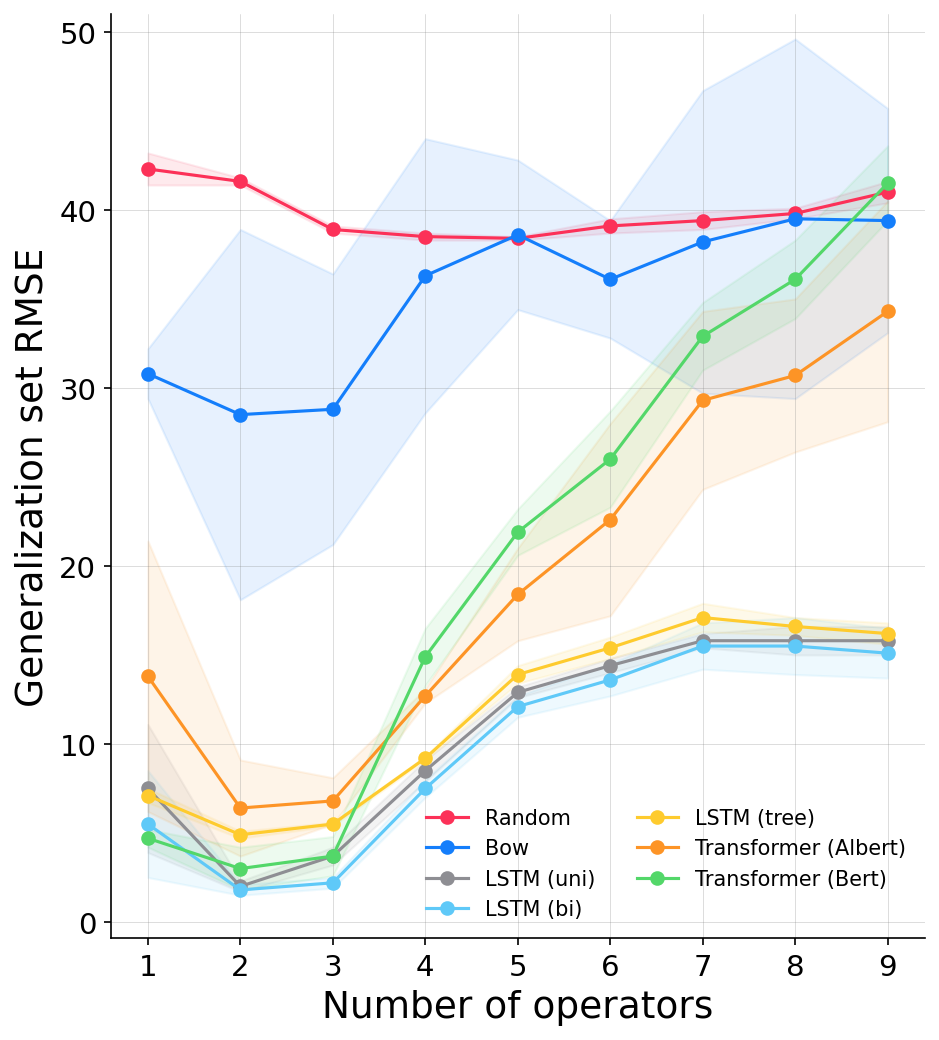
\includegraphics[width=\textwidth]{images/productivity_v2.png}
        \caption{}
        \label{fig:productivity}
    \end{subfigure}
    \hfill
    \begin{subfigure}[b]{7.52cm}
        \centering 
        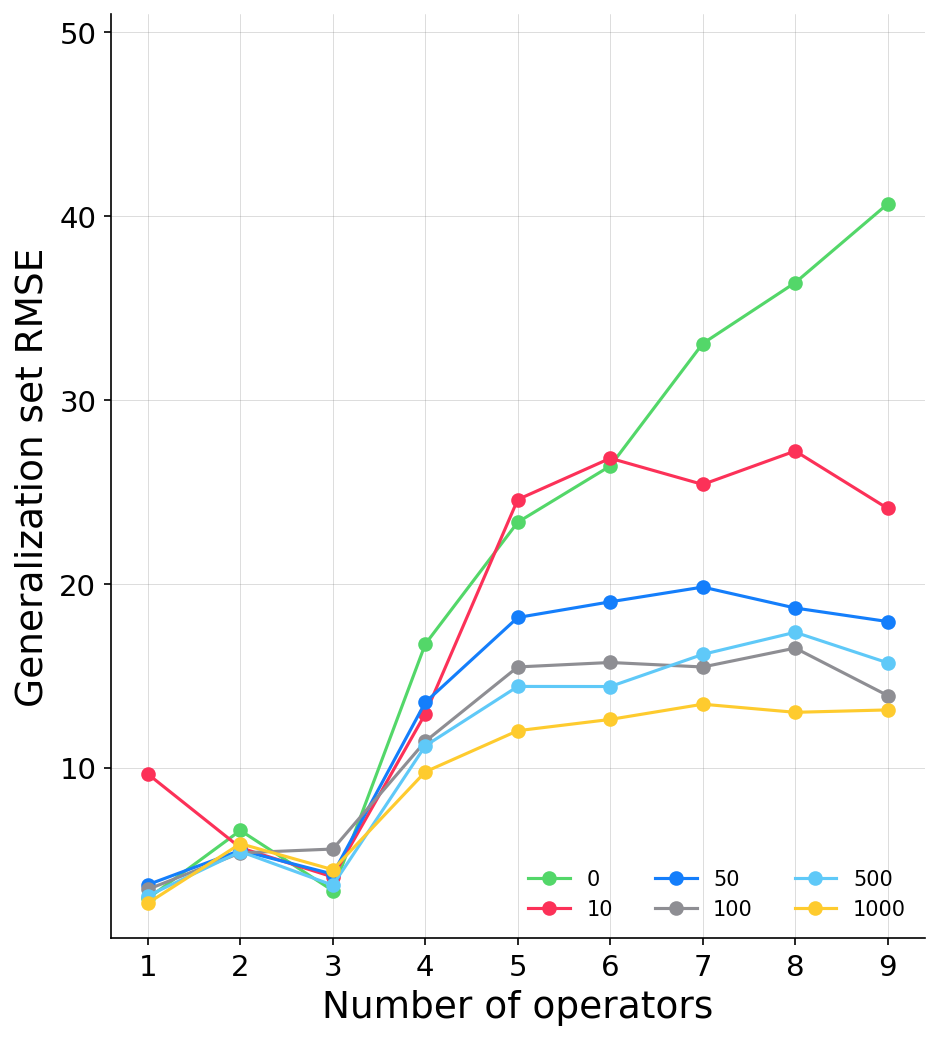
\includegraphics[width=\columnwidth]{images/productivity-exposition_v2.png}
        \caption{}
        \label{fig:productivity-exposition}
    \end{subfigure}
    \caption{Evolution of the RMSE on the productivity generalization set given the number of operators. (a) We report the mean evolution over 4 runs for each encoder (standard deviation in light). As detailed in Table~\ref{table:paritions}, expressions from the in-domain set have 2.8 operators on average. (b) For the \textsc{Bert}-based encoder, we expose the model to a proportion of generalization examples during training.}
\end{figure*}

Since we use generated arithmetic expressions, it is easy to control their fine-grained properties. We investigate further the influence of parameters for each partition. As part of our study, we observe how the complexity of the examples impacts compositional abilities and how we can enhance them by modifying model hidden size or exposing models to generalization examples during training.

\subsubsection{Impact of the expression's complexity}

\paragraph{Complexity of compositional operations} As observed in Table~\ref{table:results-main}, all models perform reasonably well on the random partition. Yet, this performance might be heterogeneous across examples. We decompose the examples according to the type of operations involved. We consider expressions containing at least one addition sign (\textbf{Add}), at least one multiplication sign (\textbf{Mul}), only addition sign(s) (\textbf{Only Add}), only multiplication sign(s) (\textbf{Only Add}) and at least one multiplication and addition sign (\textbf{Add and Mul}). We present the performance given this stratification in Figure~\ref{subfig:random-study}.

Arithmetic expressions involving at least one addition operator obtain better results. Multiplications, on the other hand, tend to make the task harder. In expressions that involve addition and multiplication, there may be cases where multiplication should take precedence over addition, and for which computation order matters. Surprisingly, these expressions reach performance in line with expressions containing only one operator type. 

\paragraph{Number of operators for productivity} Productivity is notoriously hard \parencite{kim_20, hupkes_20, baroni_19}. We also observe that neural networks struggle to generalize to longer expressions in our main results Table~\ref{table:results-main}. In Figure~\ref{fig:productivity}, we decompose the productivity generalization set according to the number of operators per expression and plot the evolution of the RMSE. In line with intuition, performance declines as the number of operators grows. This evolution is not uniform across architectures: LSTM architectures generalize better to long sequences. 
% Regarding transformers, tying parameters also help for productivity. Encoder based on \textsc{Albert} over perform the on based on \textsc{Bert} for large operator numbers.

\begin{figure*}[htb!]
    \centering
    \begin{subfigure}[b]{7.52cm}
        \centering
        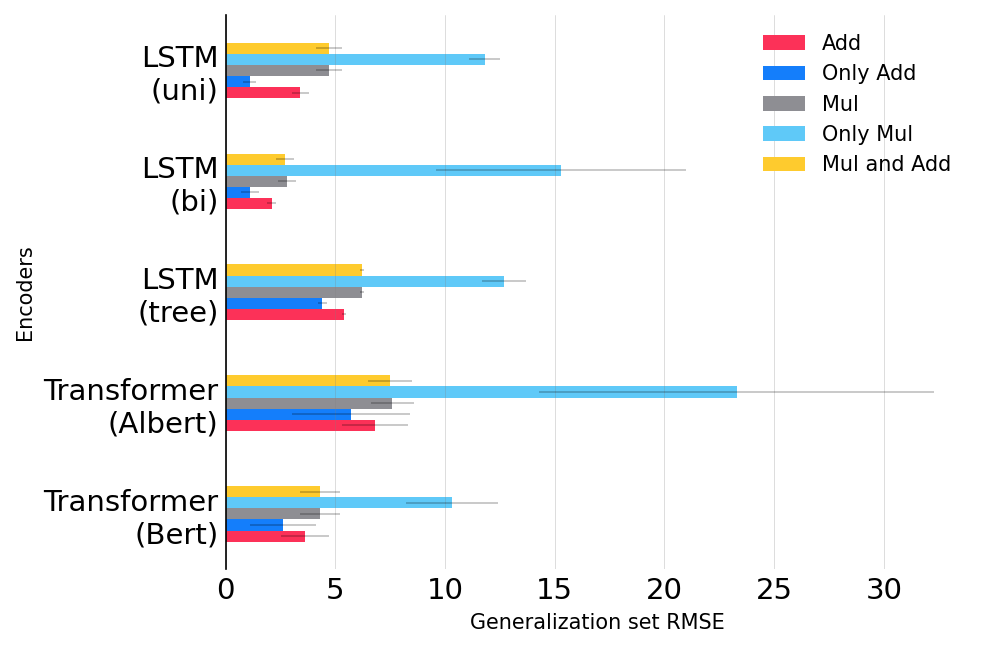
\includegraphics[width=\textwidth]{images/random-study_v3.png}
        \caption{}
        \label{subfig:random-study}
    \end{subfigure}
    \hfill
    \begin{subfigure}[b]{7.52cm}  
        \centering 
        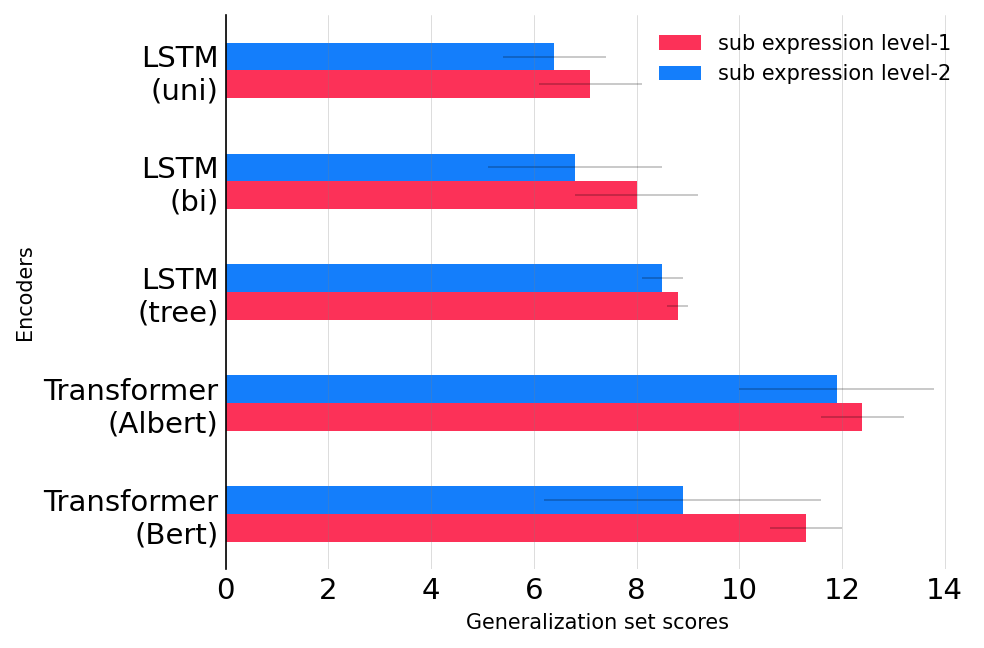
\includegraphics[width=\textwidth]{images/localism-study_v3.png}
        \caption{}
        \label{subfig:localism-study}
    \end{subfigure}
    \vskip\baselineskip
    \begin{subfigure}[b]{7.52cm}   
        \centering 
        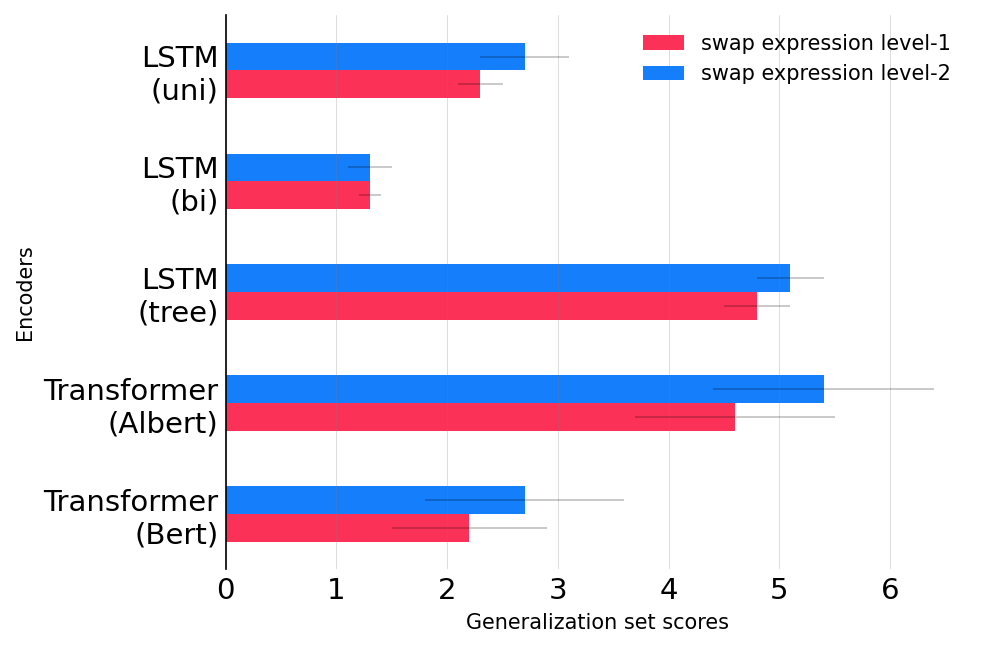
\includegraphics[width=\textwidth]{images/substitutivity-study_v3.png}
        \caption{}
        \label{subfig:substitutivity-study}
    \end{subfigure}
    \hfill
    \begin{subfigure}[b]{7.52cm}
        \centering 
        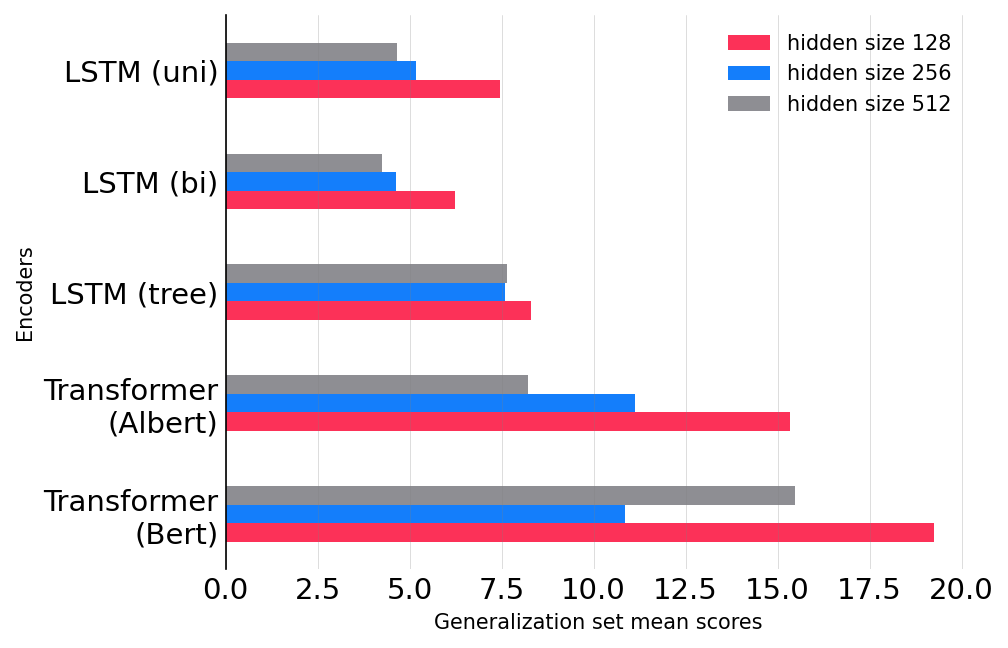
\includegraphics[width=\textwidth]{images/hidden-size-study_v2.png}
        \caption{}
        \label{subfig:hidden-size}
    \end{subfigure}
    \caption{Impact of the expression complexity and model hidden size on the compositional performances. (a) We decompose the expressions from the random partition given the type of operators involved. (b) We decompose the expressions from the local partition given the number of sub-expression evaluated (c) We decompose the expressions from the substitutivity partition given the number of swaps (d) We compare the impact of the model hidden size on the average mean generalization score for each partition. For this specific analysis, we observe transformers might struggle to converge. We adapt the training procedure by increasing the warm-up to 1000 steps with no decay.}
\end{figure*}

\paragraph{Number of swaps} For substitutivity, we organize the dataset given tuples of swapped expressions. During evaluation, we pair each expression with an expression from the same tuple and we compare the predicted value between the two. As illustrated in Figure~\ref{fig:loc_prod}, we can rank all expression pairs given the number of swaps necessary to generate one given the other. For example, given the expression $2 + 2 \times 4$ we can generate $2 + 4 \times 2$ with only one swap. We refer to this pair as level-1. We need to perform two swaps to generate $4 \times 2 + 2$: we refer to the pair as level-2. Figure~\ref{subfig:substitutivity-study} decomposes the results from the substitutivity partition given these levels. Encoders tend to reach better performance for expression pairs with only one swap. 
% This points the impact of local variations towards compositional abilities.

\paragraph{Complexity of local evaluations} For the localism partition, we organize the dataset given tuples of sub-expressions. As illustrated in Figure~\ref{fig:loc_prod}, we can rank all expression pairs given the number of evaluated intermediate operators between the two. For example, given the expression $2 + 5 + 2 \times 4$, we evaluate only the first addition operator to generate $7 + 2 \times 4$. We refer to the expression pair as level-1. If also we evaluate the multiplication operator, we obtain $7 + 8$. We then refer to the expression pair as level-2. We compare the results on the Localism partition by decomposing generalization examples given this level. We aim to better quantify how local the encoder performs composition operations. Surprisingly, Figure~\ref{subfig:localism-study} shows that level-2 expression pairs reach better scores for all encoders. We hypothesize that expressions with intermediate evaluated operators are shorter and therefore reach higher evaluation scores.

\subsubsection{Enhancing model compositional abilities}

\paragraph{Model hidden size} The number of parameters indubitably boosts model performance. We analyze here whether the number of parameters can also leverage performance for out-of-domain generalization. We compare embedding and hidden sizes of \numprint{128}, \numprint{256}, and \numprint{512} and observe the impact on the out-of-domain generalization performances. We plot in Figure~\ref{subfig:hidden-size} the mean score for each partition given each encoder. For all encoders, we observe that the number of parameters benefits compositional generalization. On average, all models indeed reach the lowest RMSE on the generalization set with 512 hidden and embedding size than 128.

\paragraph{Exposition during training} We study how to increase out-of-domain generalization for productivity. We consider exposing the model to a small number of out-of-domain examples during training. We randomly include between \numprint{10} and \numprint{1000} expressions from the generalization set in the training samples. These expressions are then removed from the generalization set. In Figure~\ref{fig:productivity-exposition}, we plot the evolution of RMSE on the productivity extrapolation set given the number of operators per expression for the transformer encoder. 

%We observe the impact of the exposition on training samples. 
With our dataset, only a minimal number of out-of-domain examples exposed during training may not be sufficient to trigger generalization during inference. Even by including a large portion, between \numprint{500} and \numprint{1000} expressions, we still observe a significant performance drop for expressions with a large number of operators. With this configuration, the transformer falls short of the trend obtained with the sequential LSTM.

% \subsection{Embeddings}
% \label{subsec:embeddings}

% We also try to learn the number embeddings from scratch. We compare the global scores for the LSTM (uni) using either pre-trained DICE or randomly initialized but updated embeddings.


% We evaluate the learned embeddings on the Benchmark from \textcite{wallace_19} to evaluate their quality.

% \subsection{Positional Embeddings}
% \label{subsec:positional-embeddings}

% As observed in many studies \parencite{wallace_19, kim_20, csordas_21}, the configuration of the positional embeddings for the transformers are crucial. Relative positional embeddings might be used. We choose to use the setup from \textcite{wallace_19}. During training, we add some random padding in the expressions. For examples, the expression \textsc{[CLS]} $\times$ 4 $+$ 5 2 \textsc{[SEP]} would become \textsc{[CLS] [PAD] [PAD] [PAD]}$\times$ 4 $+$ 5 2 \textsc{[SEP]}. Positional embeddings from latter position are thus trained. Moreover, the encoder cannot rely on the absolute character positions to solve the task. We compare the global score with and without this specific configuration for the encoder based on \textsc{Bert} architecture.

% \begin{figure}[htb!]
%     \centering
%     \includegraphics[width=\columnwidth]{figures/productivity-exposition.png}
%     \caption{Evolution of the RMSE test given the number of operators.}
%     \label{fig:productivity}
% \end{figure}

% \section{Discussion}
% \label{sec:discussion}

% Evaluating model compositional properties on arithmetic expressions is not directly transferable to assess the ability of model to learn composition rules from language. Language structure exhibit indeed completely distinct properties \bccomment{which ones ?}.

% The set of composition operations is indeed completely different. However, while such properties might have distinct manifestation, they might be declined for both universes.

% \subsection{Conclusion}
% \label{sec:conclusion}

% % We introduced CobA, a dataset of arithmetic expressions. The dataset is specifically designed to evaluate model compositional properties. We partition the dataset into multiple in-domain and generalization sets. Since arithmetic is defined by explicit and formal rules, we can precisely control the properties of the generated expressions. For each partition, we therefore carefully control the distribution of the two sets by introducing specific statistical differences. We use these partitions to evaluation specific compositional aspects that also apply to the study of human language. We hope our work may help better characterize compositional abilities to design more efficient encoders: either by adapting architectures or training methods.
% We \bcomment{introduce}{describe} CobA, a dataset \bcomment{to study compositionality}{} of arithmetic expressions. The dataset is specifically designed at evaluating model compositional properties. We partition the dataset into multiple in-domain and generalization sets. As arithmetic follows explicit and formal rules, we can precisely control the properties of the generated expressions and, consequently, the statistical properties of the sets. For each partition, we introduce controlled differences between the distribution of the two sets. We then study the ability of models to evaluate out-of-domain expressions from the generalization set, by learning compositional rules from the in-domain set. We build partitions to evaluate compositional properties (localism, substitutivity, productivity, and systematicity) that also apply to the study of human language. We hope our work may help better characterize compositional abilities to design more efficient encoders: either by adapting architectures or training methods.

% We use the dataset to compare encoders with distinct structures: transformers, recurrent or tree-structured models. In general, models are robust toward the introduction of paraphrases (substitutivity) and can perform recursive evaluation of sub-components (localism). Yet, transformers struggle to generalize to longer sequences (productivity) or to combine known parts to form new sequences (systematicity). We perform an in-depth analysis and make observations in line with intuition. Models struggle with complex expressions, involving more symbols, more complex structure, or more operators types. We slightly enhance the compositionality degree by adapting the number of parameters or the exposition to generalization expressions. Yet the encoder architecture is the key parameter in our study. 

\section{Conclusion and future work}

% By carefully selecting expressions from the in-domain and generalization sets, we introduce controlled differences between the two sets.
% We show that models achieve competitive performance on a random partition, for which there is no controlled difference. Yet, for partitions requiring compositional extrapolation, performances drastically decrease for most encoder architectures. 
This chapter examined how the model structure impacts its degree of compositionality. We conducted experiments on two datasets with annotations allowing us to analyze better model performances: a NLI task presenting specific syntactic or lexical properties; CobA, a dataset of arithmetic expressions specifically designed to evaluate compositional properties along with four aspects: localism, substitutivity, productivity, and systematicity. We compared various structured models and outlined their strengths and weaknesses, given the properties of interest for each task. As a result of both experiments, we observed heterogeneity of results across both properties and model structures, suggesting that structure influences the way and type of information models capture.

On the NLI task, pre-trained \bert models seem to encode information not captured by others. Indeed, models using \bert embeddings almost systematically achieve a better score. However, cases remain for which structured models can improve the performance of stand-alone contextualized embeddings. In such cases, syntactic information may not be fully encoded in \bert. We identified a specific transformation that replaces words with the semantic opposite. For such transformation, \bert contextualized embeddings lead to surprisingly low performances. Finally, we identified cases for which all models fail, particularly for the word scrambling transformation. 

Regarding CobA, models are, in general, robust toward introducing paraphrases (substitutivity) and can perform a recursive evaluation of sub-components (localism). Yet, transformers struggle to generalize to longer sequences (productivity) or combine known parts to form new sequences (systematicity). This difficulty increases with the complexity of the expression and structure, the number of symbols and operator types. 

In both experiments, we observe that results could be slightly improved by balancing the training set distribution and adapting the number of parameters or the exposition to generalization expressions. In both cases, there is still room for improvements in fully capturing compositional abilities and common sense knowledge within NLP models.
